\documentclass[]{tufte-book}

% ams
\usepackage{amssymb,amsmath}

\usepackage{ifxetex,ifluatex}
\usepackage{fixltx2e} % provides \textsubscript
\ifnum 0\ifxetex 1\fi\ifluatex 1\fi=0 % if pdftex
  \usepackage[T1]{fontenc}
  \usepackage[utf8]{inputenc}
\else % if luatex or xelatex
  \makeatletter
  \@ifpackageloaded{fontspec}{}{\usepackage{fontspec}}
  \makeatother
  \defaultfontfeatures{Ligatures=TeX,Scale=MatchLowercase}
  \makeatletter
  \@ifpackageloaded{soul}{
     \renewcommand\allcapsspacing[1]{{\addfontfeature{LetterSpace=15}#1}}
     \renewcommand\smallcapsspacing[1]{{\addfontfeature{LetterSpace=10}#1}}
   }{}
  \makeatother

\fi

% graphix
\usepackage{graphicx}
\setkeys{Gin}{width=\linewidth,totalheight=\textheight,keepaspectratio}

% booktabs
\usepackage{booktabs}

% url
\usepackage{url}

% hyperref
\usepackage{hyperref}

% units.
\usepackage{units}


\setcounter{secnumdepth}{2}

% citations
\usepackage{natbib}
\bibliographystyle{apalike}

% pandoc syntax highlighting

% longtable
\usepackage{longtable,booktabs}

% multiplecol
\usepackage{multicol}

% strikeout
\usepackage[normalem]{ulem}

% morefloats
\usepackage{morefloats}


% tightlist macro required by pandoc >= 1.14
\providecommand{\tightlist}{%
  \setlength{\itemsep}{0pt}\setlength{\parskip}{0pt}}

% title / author / date
\title{Cell Atlas}
\author{Jensen Lab}
\date{2020-02-14}

\usepackage{booktabs}
\usepackage{amsthm}
\makeatletter
\def\thm@space@setup{%
  \thm@preskip=8pt plus 2pt minus 4pt
  \thm@postskip=\thm@preskip
}
\makeatother

\begin{document}

\maketitle



{
\setcounter{tocdepth}{1}
\tableofcontents
}

\chapter{Introduction}\label{introduction}

\chapter{Envelope}\label{envelope}

\section{Mycoplasma genitalium}\label{mycoplasma-genitalium}

The fundamental unit of life is the cell -- a contained self-replicating
assembly. For many species, including all Bacteria and Archaea, the
organism consists of a single cell. And for nearly all species, no
matter how many cells an organism eventually contains (probably around
10 trillion in your case), it started life as a single cell. As you'll
see, the details of these cells vary, but every cell on Earth is the
same at heart -- a DNA-based replicator machine built from just four
macromolecules: nucleic acids, proteins, lipids and carbohydrates.

Imagine that you're a structural engineer tasked with building one of
these cells. What's the first step? Let's start with the container. No
matter what the first self-replicating molecules were (likely RNA), they
didn't constitute a cell until they became packaged in a container.
You'd probably want a flexible container that allowed you to sort a
subset of molecules from the environment. Evolution agrees. All cells
are enclosed by a selectively permeable membrane, made of lipids and
proteins \protect\hyperlink{fig:2-1-1}{Schematic -- Lipid bilayer}, that
allows them to differentiate their contents from the environment. This
selectivity is a critical feature for the life of the cell
\protect\hyperlink{fig:2-1-2}{Schematic -- ATP synthase}. The
compartment enclosed by a cell's membrane is called the cytoplasm
(``cell mold'' {[}the membrane being the container that shapes the
mold{]}).

Almost all archaea and many bacteria, like these Mycoplasma genitalium
cells, are monoderms (``single skin''). This means that their cytoplasm
is enclosed by a single membrane. At the resolution of this image, the
membrane looks like a single dark line, but remember that it's really a
bilayer, as you'll see in some later images.

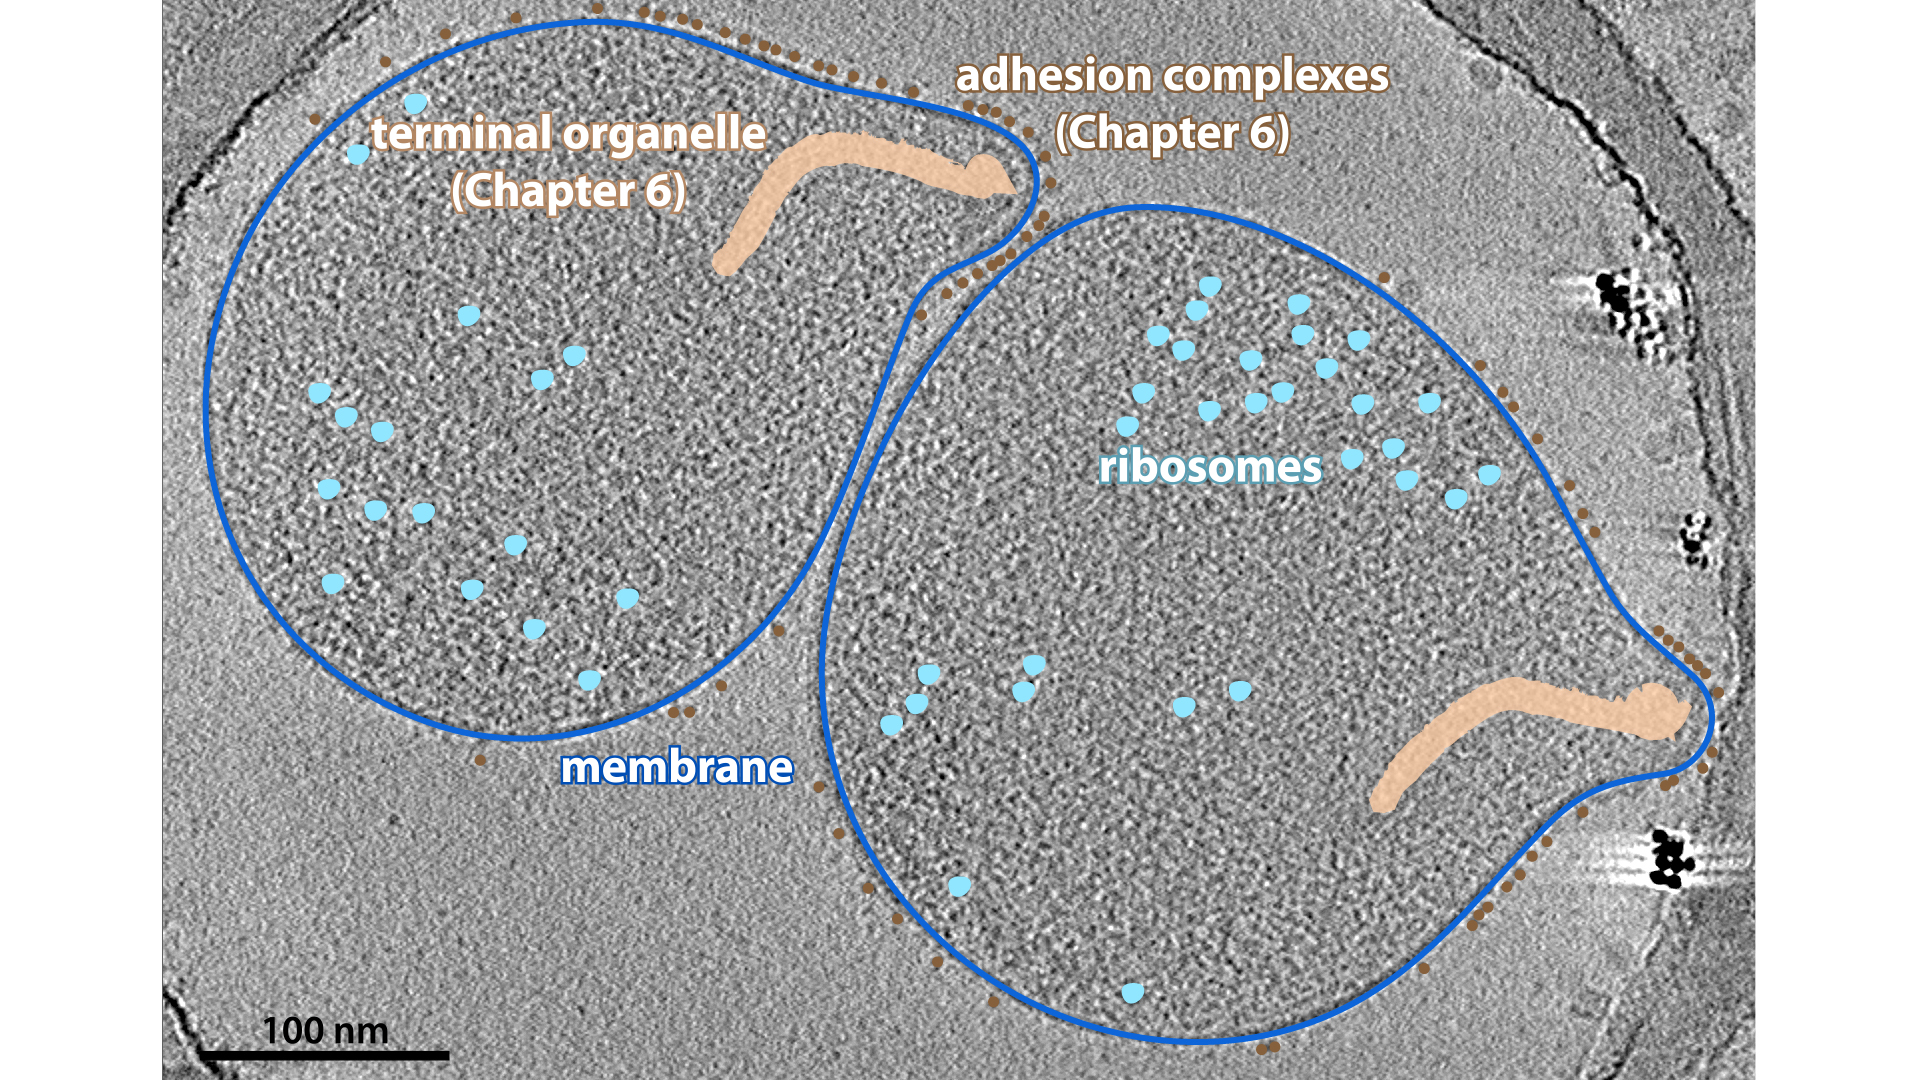
\includegraphics{img/02_static/2_1_Mgenitalium}

\begin{figure}
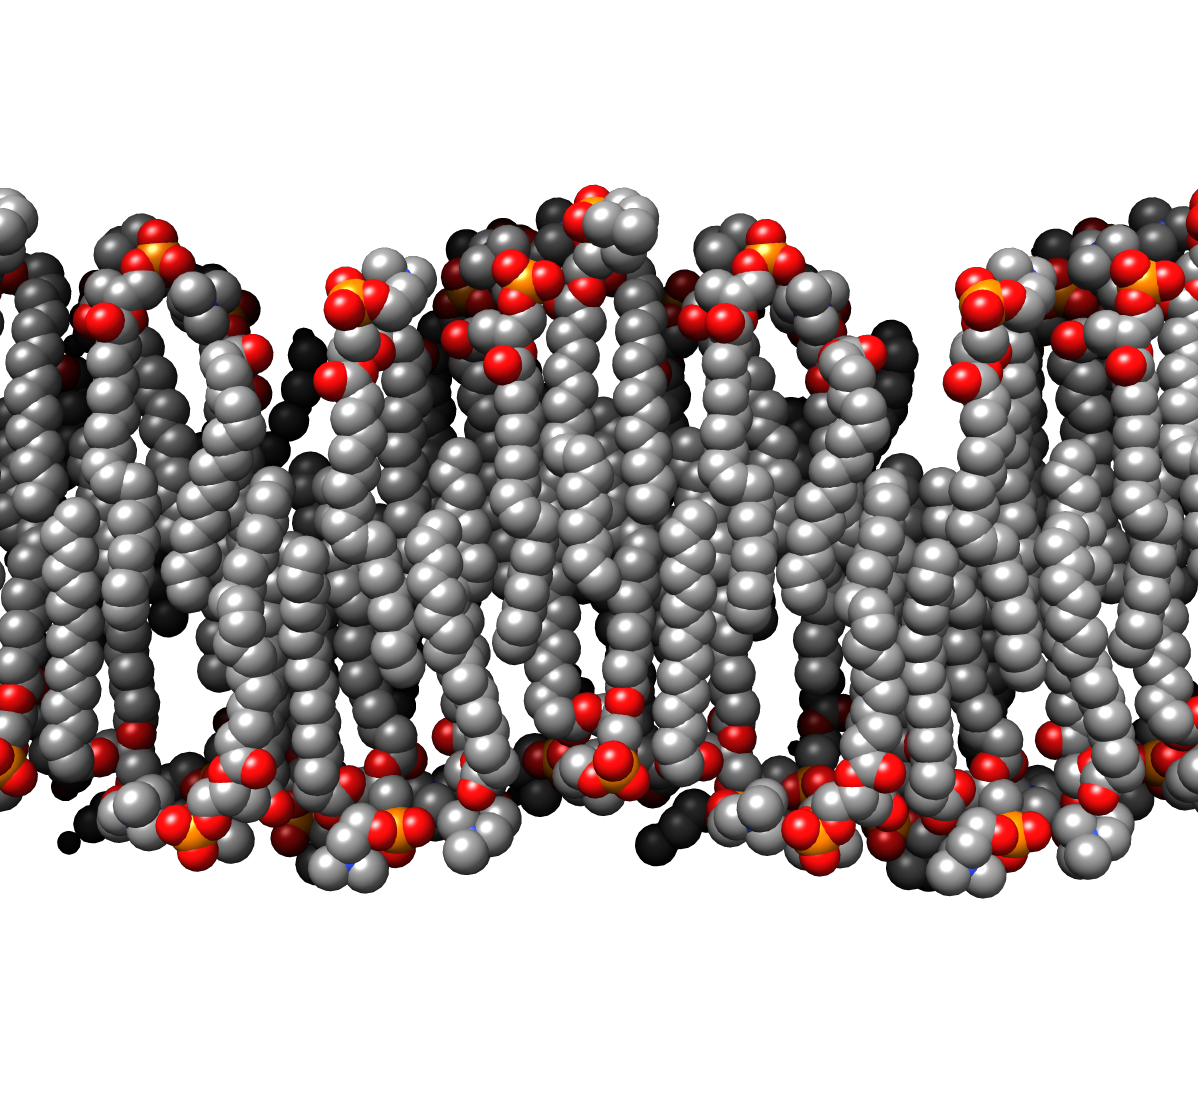
\includegraphics{img/02_schematic/2_1_1_LipidBilayer} \caption[Lipid bilayer]{Lipid bilayer}\label{fig:2-1-1}
\end{figure}

Lipids have a hydrophilic head (red/orange in the schematic) and
hydrophobic tails (gray); in water they spontaneously pack together
side-by-side to shield their tails from unfavorable interactions with
water, forming closed double-layered bags. Proteins with regions of
amino acids containing hydrophobic side groups embed these regions in
lipid bilayers. Other proteins are fused to lipids, tethering them to
the membrane. In fact, cells' ``lipid'' membranes actually constitute
roughly equal fractions of lipids and proteins. One key difference
between archaea and bacteria (and with them, eukaryotes) is the lipid
that makes up their membranes. Hybrid membranes containing both these
lipid types can be made artificially, and it's possible that the last
universal common ancestor of all cells on Earth contained both types,
with specialization later occurring in different lineages.

\begin{figure}
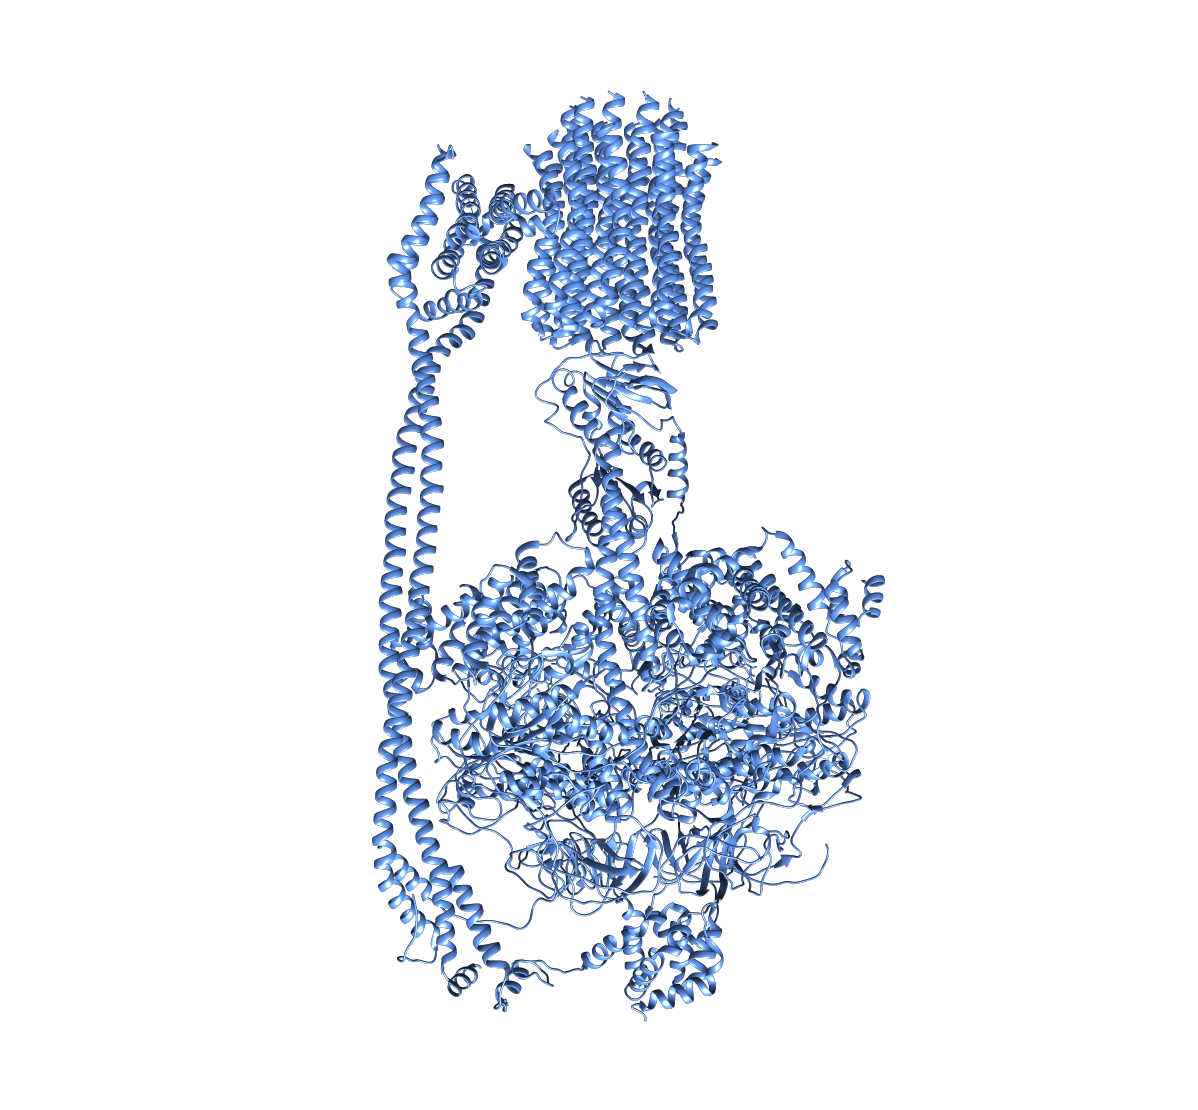
\includegraphics{img/02_schematic/2_1_2_ATPsynthase} \caption[ATP synthase and energy production]{ATP synthase and energy production}\label{fig:2-1-2}
\end{figure}

The chemical properties of lipids make membranes impermeable to ions and
large or hydrophilic molecules (but not to water). Cells take advantage
of this property to establish an ion gradient across the membrane, using
a chain of electron-carrying proteins in the membrane to pump protons
out of the cell. Protein complexes in the membrane called ATP synthases
(like this one from Escherichia coli) use the resulting ion potential to
generate energy. The machine provides a conduit for protons to flow down
their potential, producing a ``proton-motive force'' that spins the
machine's rotor, generating energy that is chemically stored in ATP, the
energetic currency of the cell.

\section{Listeria monocytogenes}\label{listeria-monocytogenes}

Being able to selectively move things into your cell enables it to do
some powerful things. It also poses a structural problem, though.
Remember that water can pass freely through the membrane, which means
that increasing the solute concentration inside relative to the
environment will cause water to rush in as well, introducing a pressure
(known as turgor pressure) on the membrane. Lipid bilayers, though, are
unable to withstand much pressure. If your cell lives exclusively in a
consistent, and fairly high-osmolarity, environment (like our bodies, in
the case of the Mycoplasma genitalium you just saw), it can balance
internal and external osmolarity to minimize turgor pressure on the
membrane. But most cells experience much more variable environments. How
can you keep your cell from bursting in such conditions?

You'll probably want to add some rigid scaffolding outside the membrane
to buttress it against turgor pressure. Nearly all bacteria do this
using a material called peptidoglycan: long stiff polymers of glycan
sugars crosslinked by short peptides into a chain-mail-like mesh. The
full scaffold of this material surrounding the cell is called its
sacculus, or cell wall. Some archaea also have cell walls, made of a
molecule similar to peptidoglycan, but chemically distinct. Most
archaea, though, rely on a different structure for support, as you'll
see later in this chapter.

In monoderm bacteria like this Listeria monocytogenes, the cell wall is
significantly thicker than the membrane. It comprises several layers of
peptidoglycan, which can't be seen individually at the resolution of
this image, so the cell wall appears as a uniformly textured layer
\protect\hyperlink{Peptidoglycan_architecture}{More: Peptidoglycan
architecture}. It's still a mystery how large molecules can pass through
this dense layer on their way to and from the cell. Not all bacterial
cell walls are chemically identical \protect\hyperlink{}{More:
Methanobacterium formicicum}. And in some conditions, cells can lose
their walls \protect\hyperlink{}{More: L-form bacteria}.

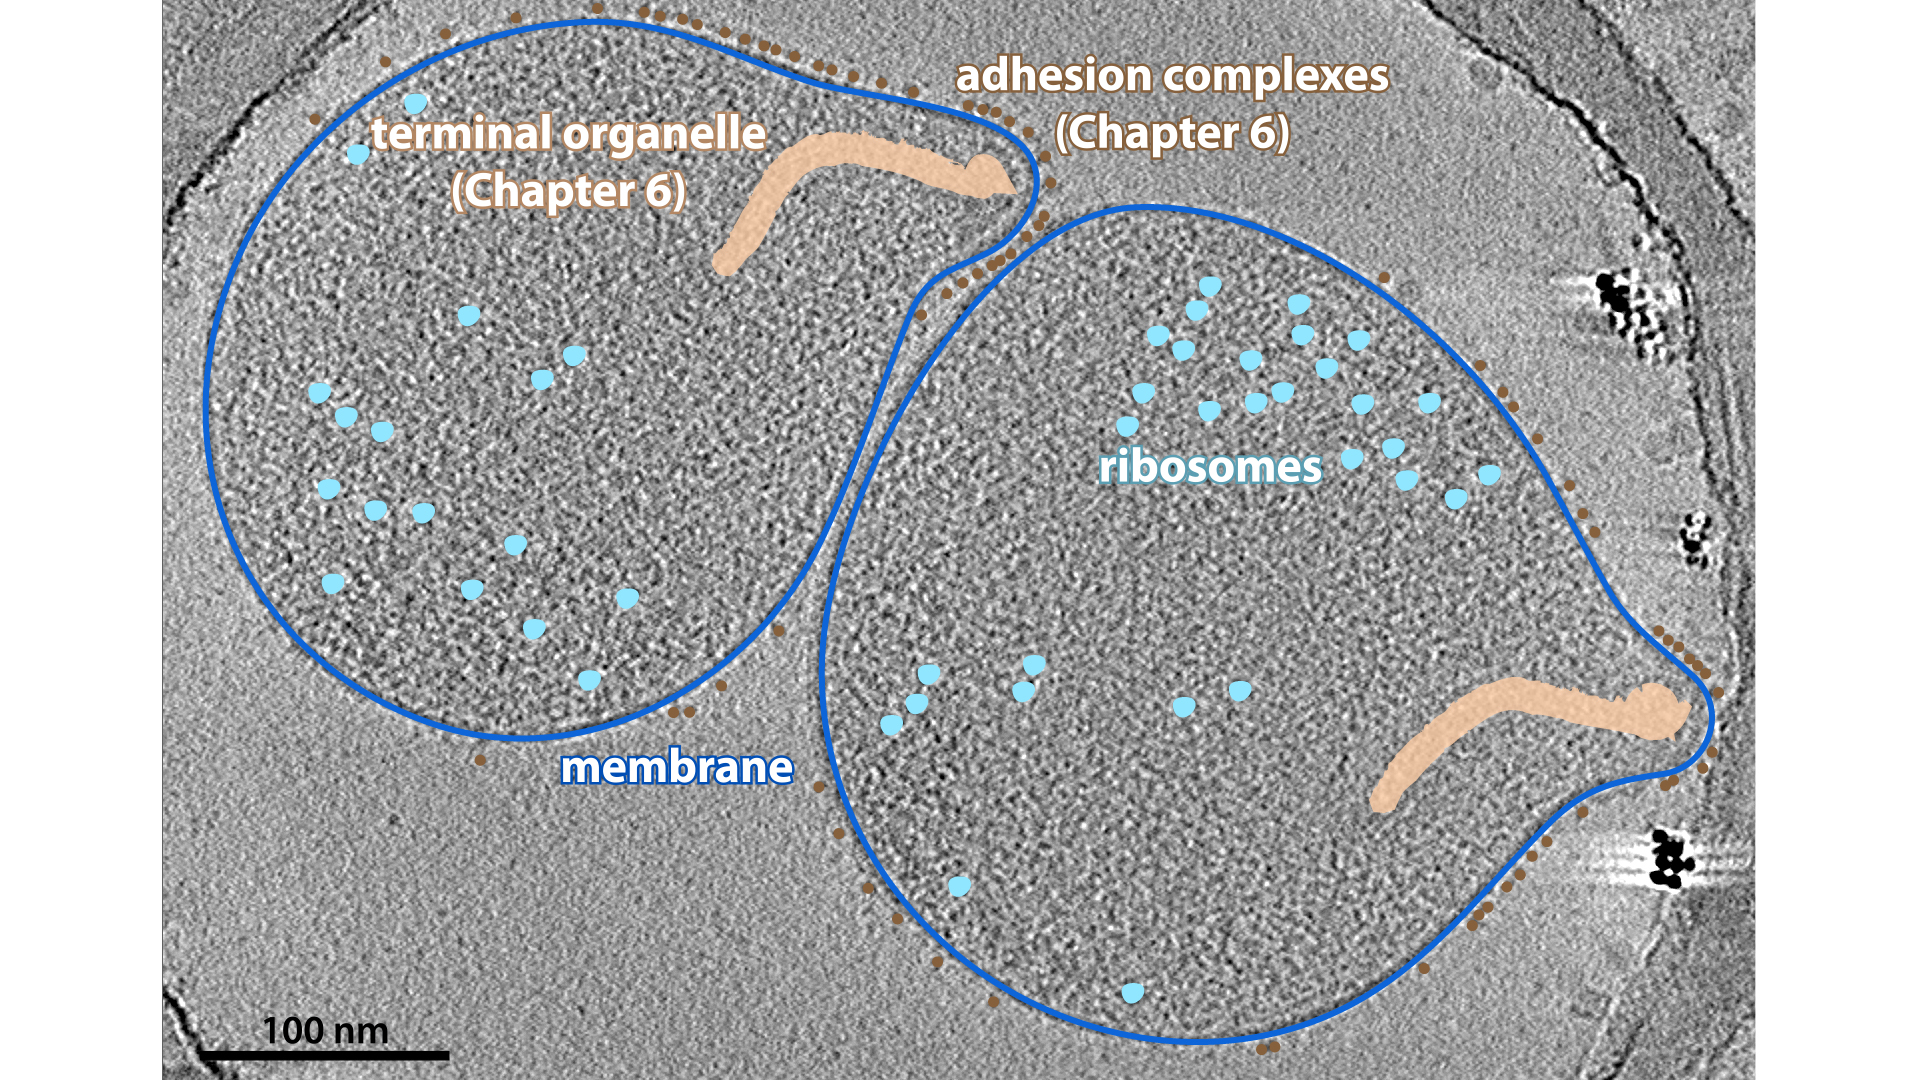
\includegraphics{img/02_static/2_1_Mgenitalium}

\hypertarget{Peptidoglycan_architecture}{\subsection{Bacillus
subtilis}\label{Peptidoglycan_architecture}}

The sacculus is so robust that it persists even after cells are lysed
and their other components digested. This sacculus isolated from a
Bacillus subtilis cell has retained its shape, simply flattening with
the release of contents and pressure from inside. By observing how these
purified sacculi rip and curl, we can infer something about the
architecture of the cell wall; we think that the long glycan strands are
oriented in hoops circling the short axis of the cylindrical cell and
the short peptide crosslinks are more or less aligned with the long
axis.

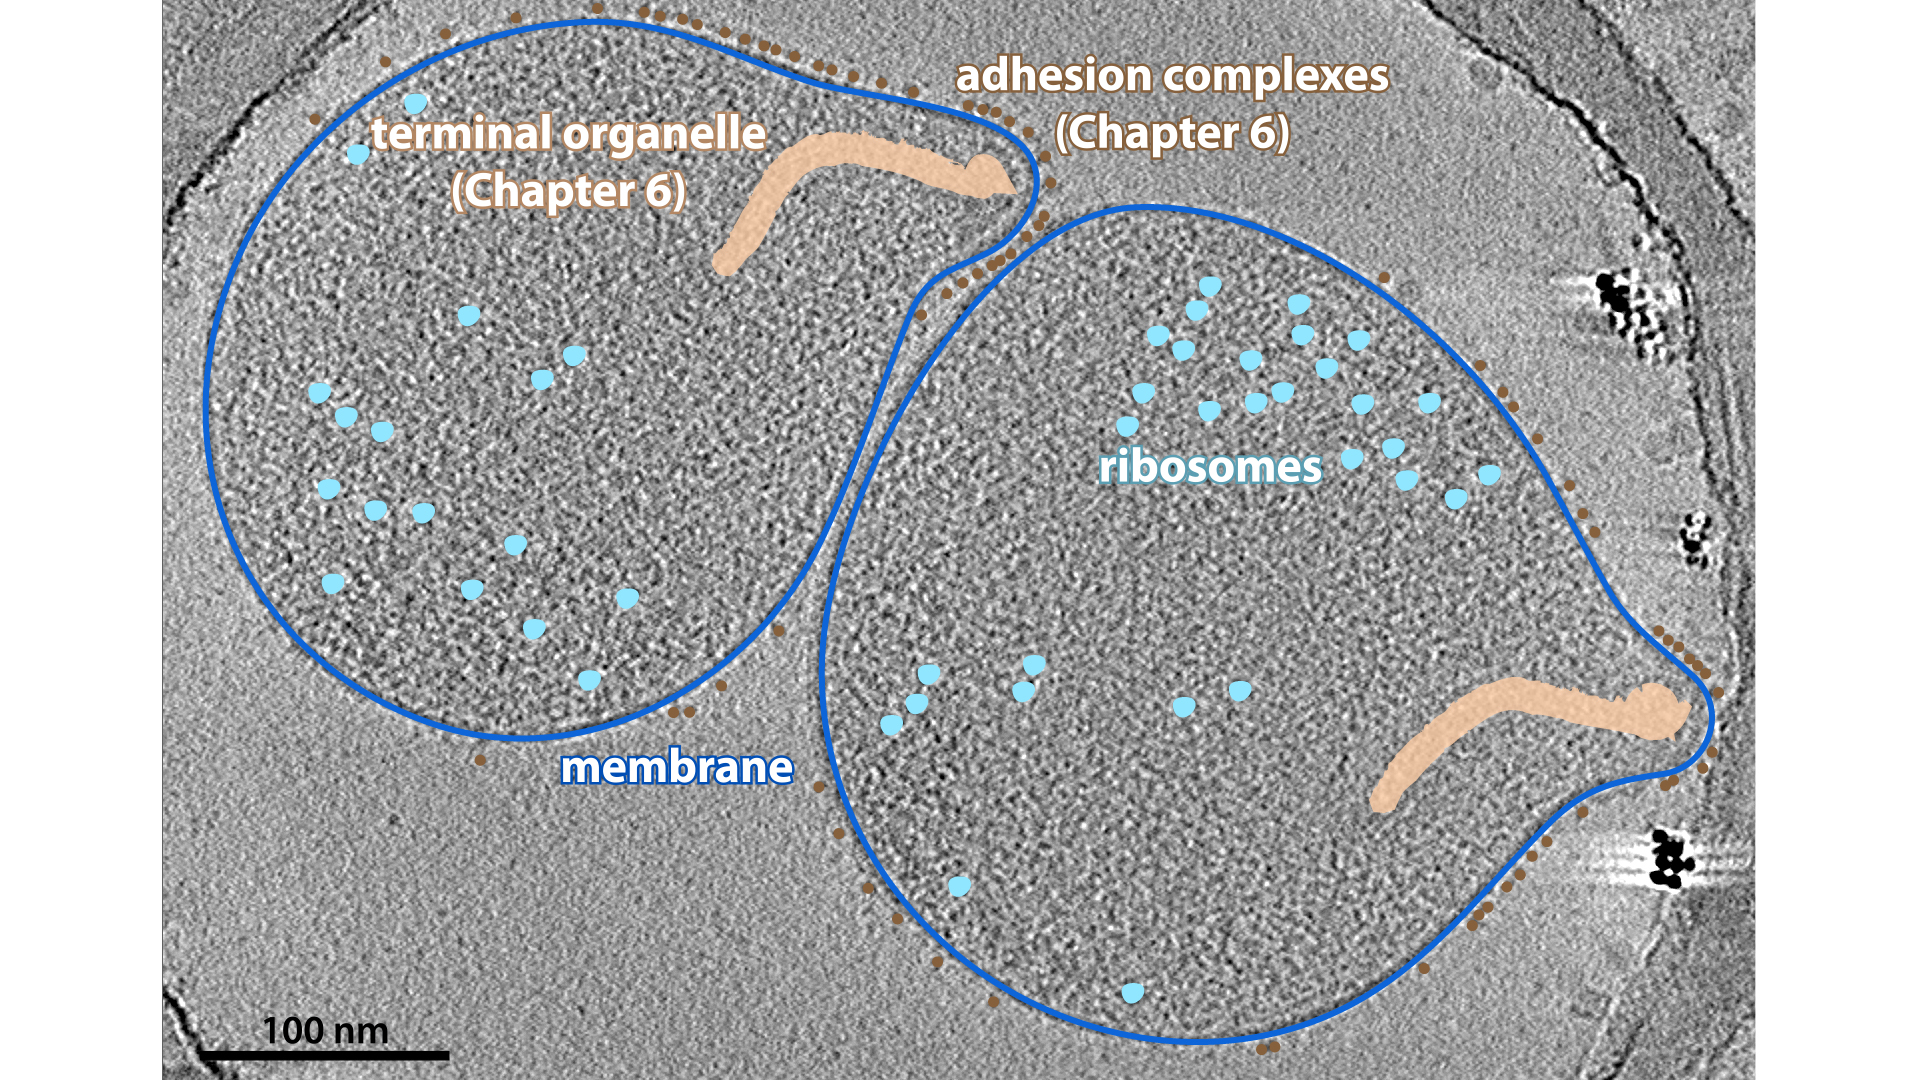
\includegraphics{img/02_static/2_1_Mgenitalium}

\begin{figure}
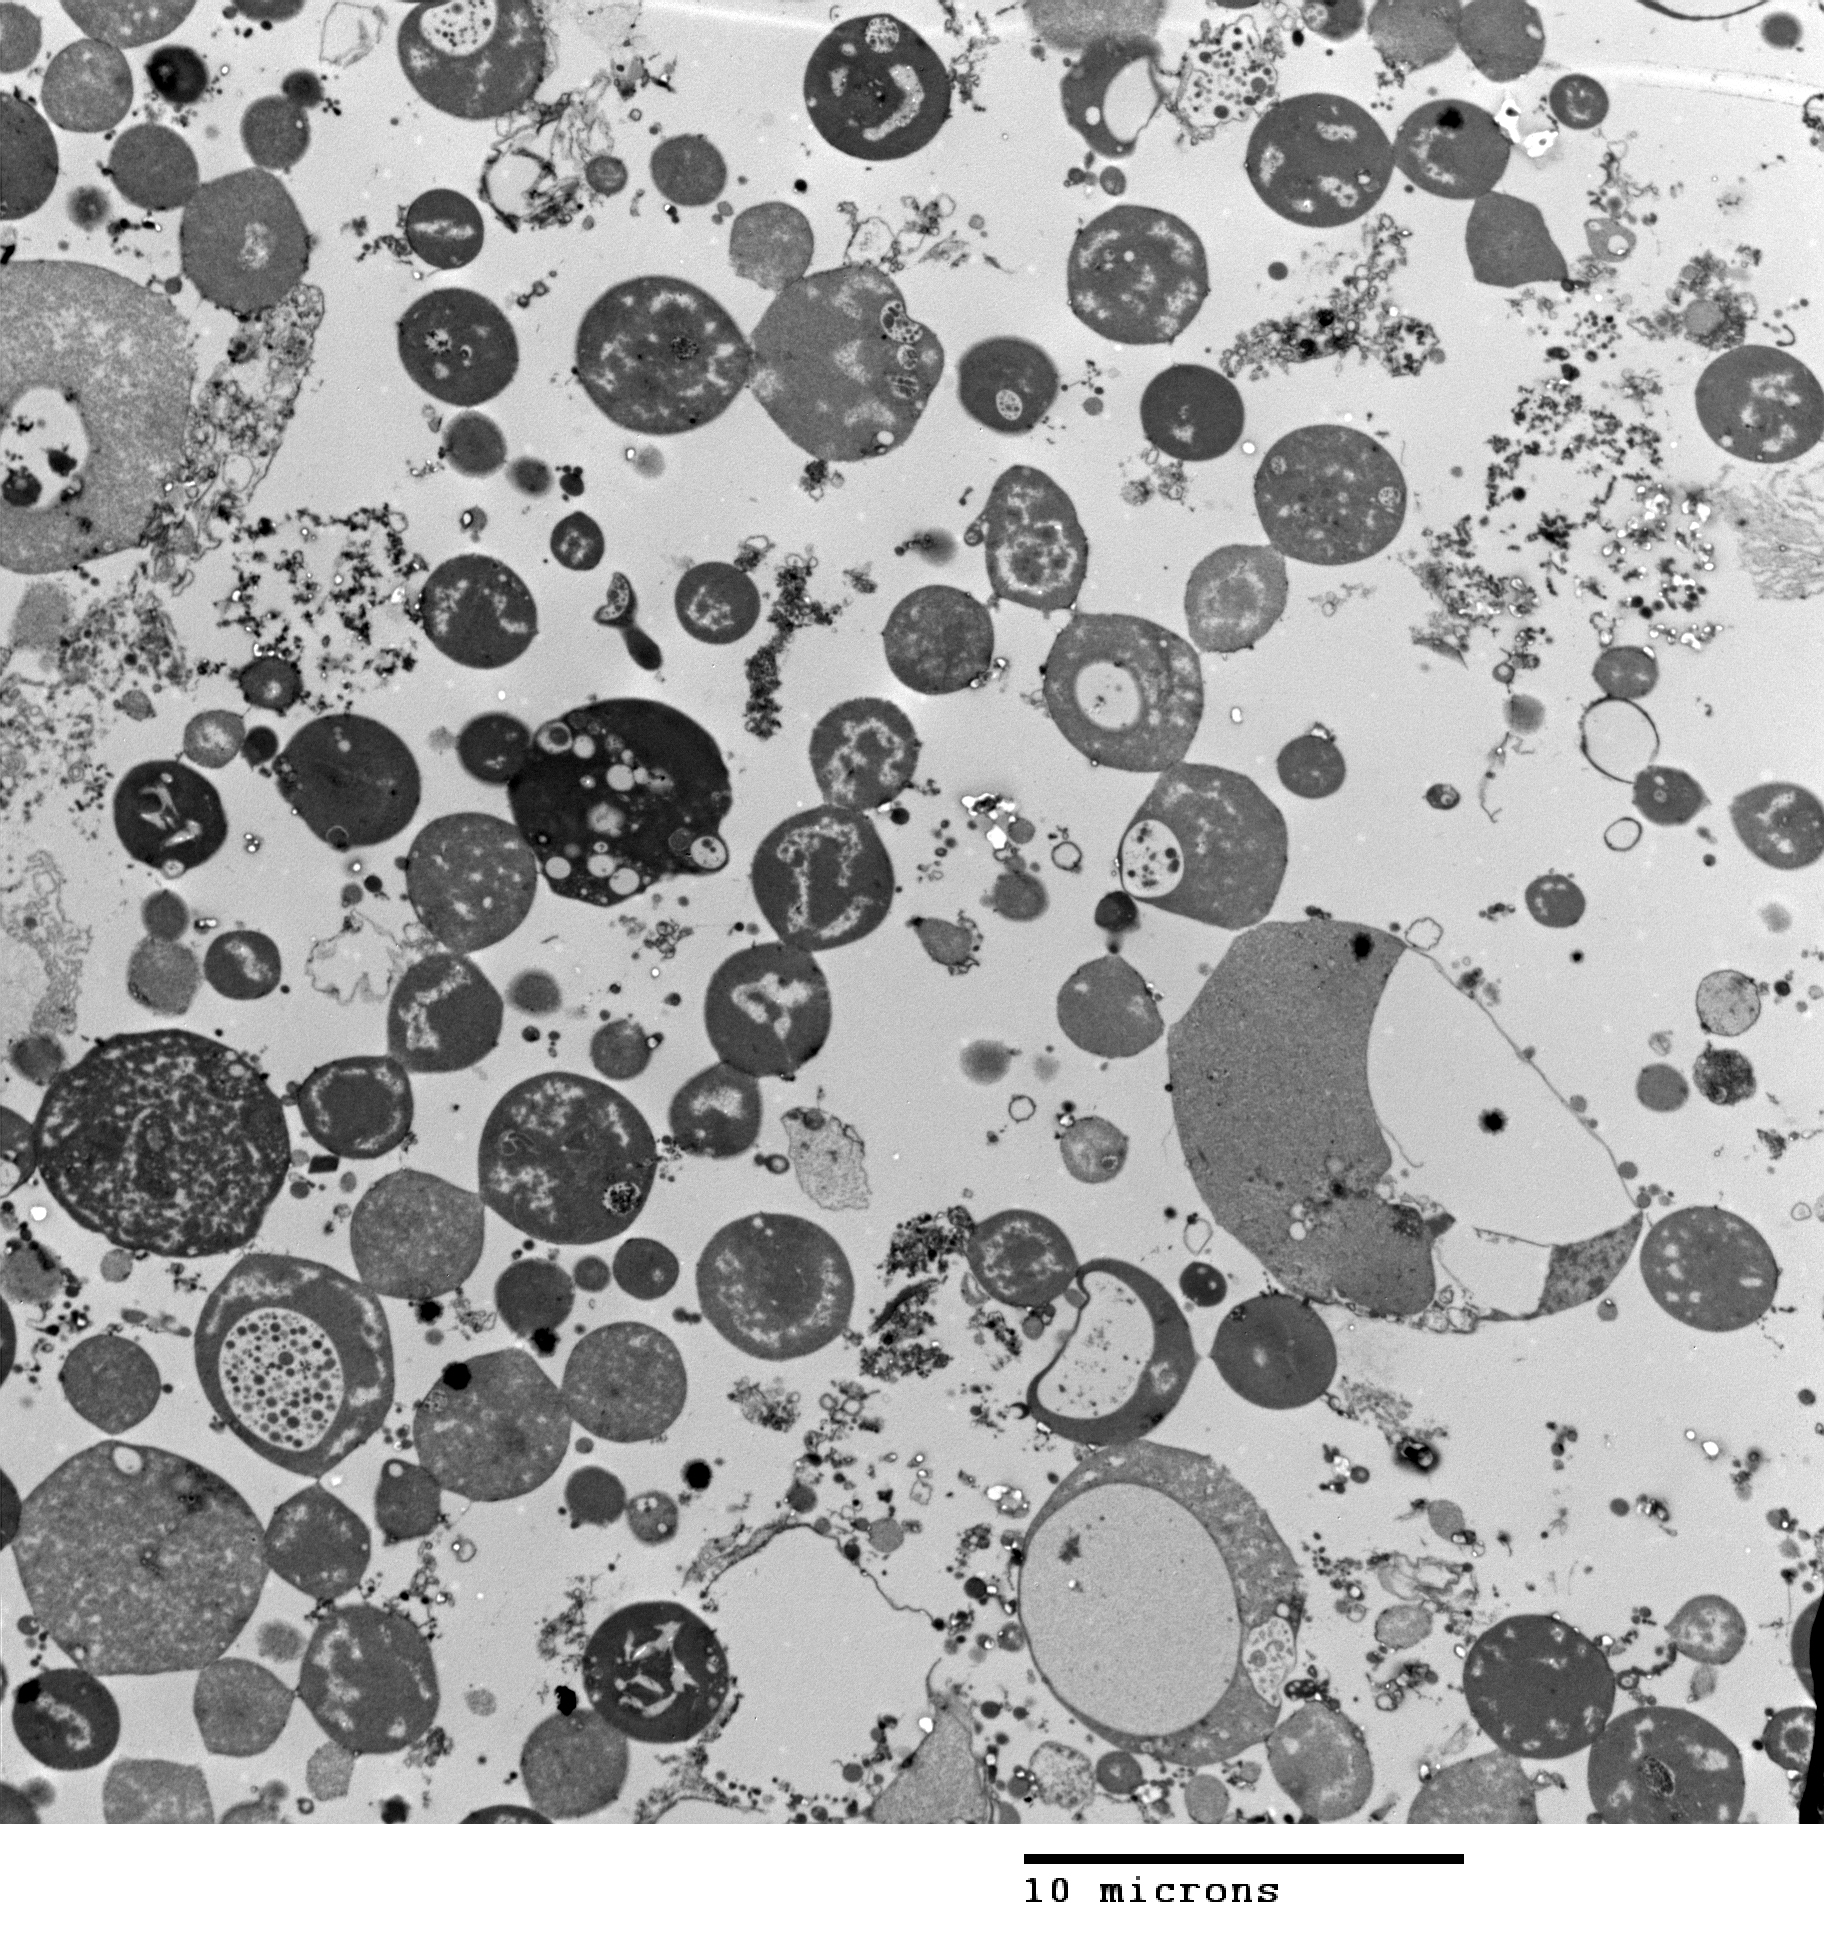
\includegraphics{img/02_schematic/2_2_1_L_form_bacteria} \caption[L-form bacteria]{L-form bacteria}\label{fig:2-2-1}
\end{figure}

There is no universal adaptation in Nature; advantages in one
environment can become liabilities in another. This concept is
exemplified by an adaptation of some bacteria which lose their cell
walls in certain conditions, such as in the presence of antibiotics (the
cell wall is a common target of antibiotics). This state is called the
L-form (named for the Lister Institute where it were discovered). As you
can see in these Bacillus subtilis, cells in this state are pleomorphic,
exhibiting a variety of sizes and shapes. As you would expect, L-form
cells are more sensitive to environmental conditions. In the lab,
they're protected from lysis by increasing the osmotic pressure of the
environment, for instance by adding sucrose. The environment in your
body, though, would have the same effect, as we discussed for Mycoplasma
genitalium. L-form bacteria are interesting for many reasons (including
human health), one of which is that they give us a fascinating window
into how early cells -- prior to the evolution of the cell wall -- might
have looked and behaved.

\section{Cupriavidus necator}\label{cupriavidus-necator}

Why stop at one membrane, though? Think about how the bacteria you've
just seen compare with eukaryotic cells. The eukaryotic cells are much
larger (maybe 100-1,000 times larger in volume), and they contain many
internal membranes that form specialized subcompartments, like the
nucleus and mitochondria. Bacteria and archaea don't have membrane-bound
organelles inside, but in fact many bacteria do create an additional
compartment outside the cell with another, outer, membrane. These
bacteria, like the Cupriavidus necator cell you see here, are called
diderms (``double skin''). The extra compartment between their membranes
is known as the periplasm (``mold between''). This antechamber contains
a unique subset of proteins, many of which function in escorting things
into and out of the main cell, as you'll see in later chapters.

Compared to the inner membrane, the outer membrane has some unique
properties. It is more permeable and not proton-tight (so it can't be
used to generate ATP). It is often asymmetric, with a different
composition of lipids and proteins in each of the two leaflets. The
outer membrane is anchored to the sacculus
\protect\hyperlink{fig:2-3-1}{Schematic -- Braun's lipoprotein}. And the
sacculus itself is different. Rather than containing many layers of
peptidoglycan like in the Listeria monocytogenes cell you just saw, the
diderm sacculus consists largely of a single-layered peptidoglycan mesh
\protect\hyperlink{Diderm_sacculus_architecture}{More: Diderm sacculus
architecture}, which you can see here as a thin line in the periplasm.
This difference in the sacculus enables a well-known bacterial
classification system: the Gram stain, which binds peptidoglycan.
Gram-positive cells, typically monoderm, contain much more peptidoglycan
than Gram-negative cells, which are typically diderm. Thinking about
this thin defense against turgor pressure underscores a major challenge
for cell growth. To insert new material, existing bonds in the sacculus
must be broken, without bursting the cell in the process
\protect\hyperlink{fig:2-3-2}{Schematic -- Sacculus remodeling}.

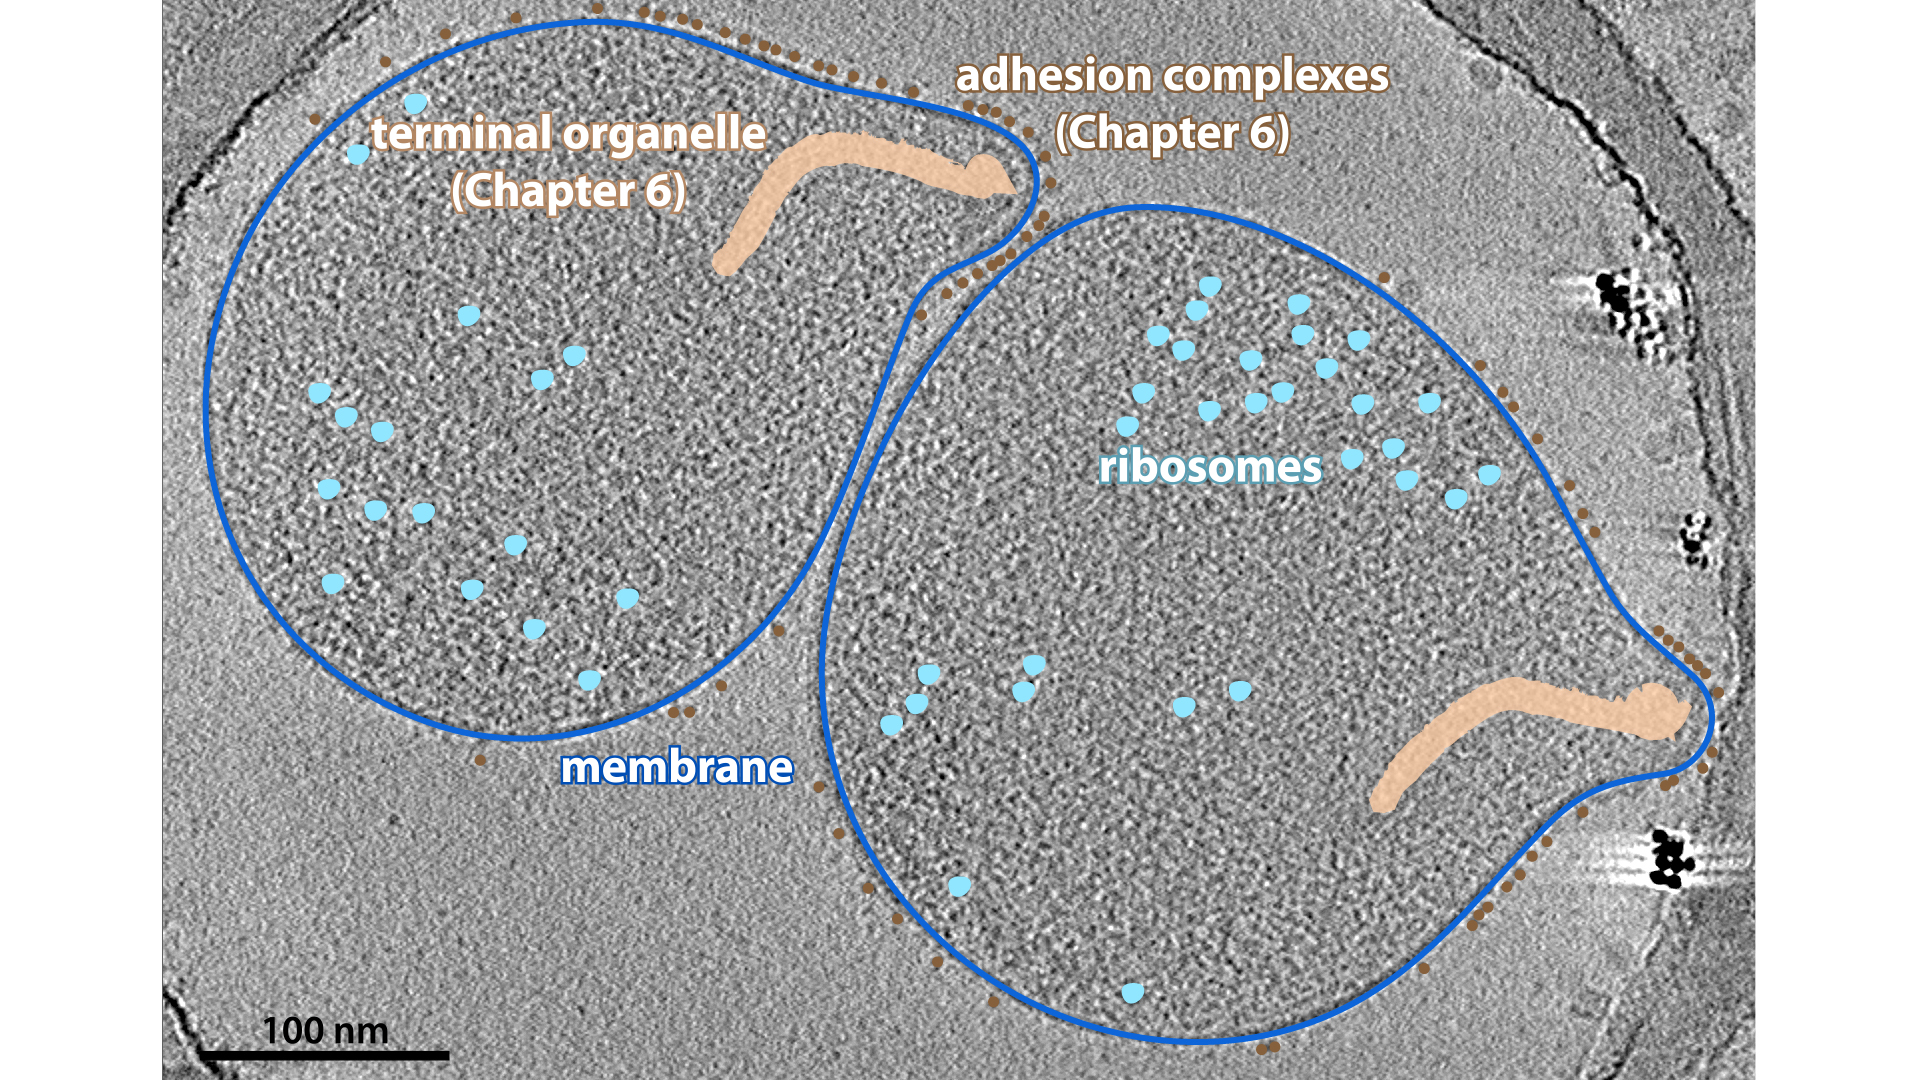
\includegraphics{img/02_static/2_1_Mgenitalium}

\begin{figure}
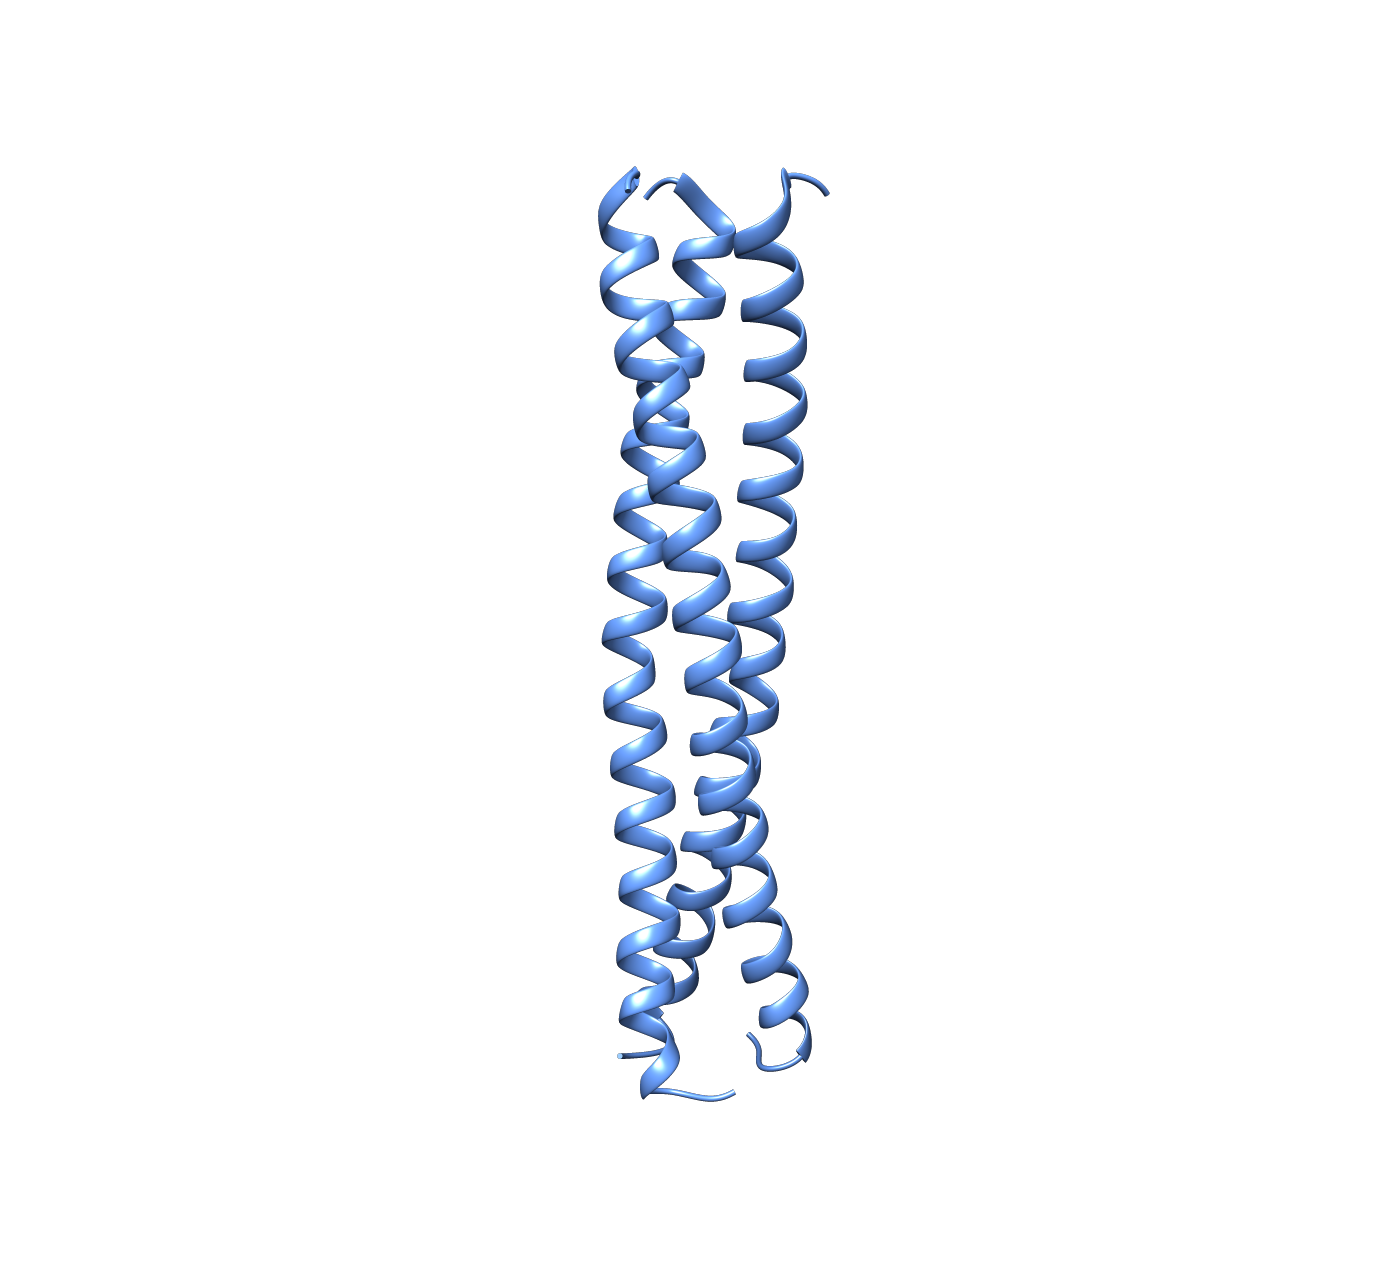
\includegraphics{img/02_schematic/2_3_1_BLP} \caption[Braun's lipoprotein]{Braun's lipoprotein}\label{fig:2-3-1}
\end{figure}

Lipoproteins are hybrid molecules, formed by covalently linked lipid and
protein pieces. The lipid allows them to embed into a membrane,
tethering the attached protein to function nearby. Braun's lipoprotein,
which is one of the most abundant molecules in the outer membrane of
cells like Escherichia coli, uses its tethered protein portion to bind
the peptidoglycan cell wall, creating a link between the outer membrane
and the cell wall (adding up, for a typical E. coli cell, to about
100,000 links). These links determine the distance between these two
components. Not all diderms use Braun's lipoprotein, though, and some
bacteria have notably labile outer membranes \protect\hyperlink{}{More:
Outer membrane lability}.

\hypertarget{Diderm_sacculus_architecture}{\subsection{Escherichia
coli}\label{Diderm_sacculus_architecture}}

Compare this diderm sacculus purified from Escherichia coli to the
monoderm sacculus on the last page. Since this one is thinner; we can
make out more details. Instead of inferring how the glycan strands are
oriented, we can now see them running around the circumference of the
cell. The main difference between the two types of sacculi seems to be
whether they have largely a single layer of peptidoglycan (diderm) or
many layers (monoderm). So even though the two cell walls look
different, their architecture is fundamentally the same. In some
circumstances, cells can even switch between the two forms, as you'll
see in Chapter 7.

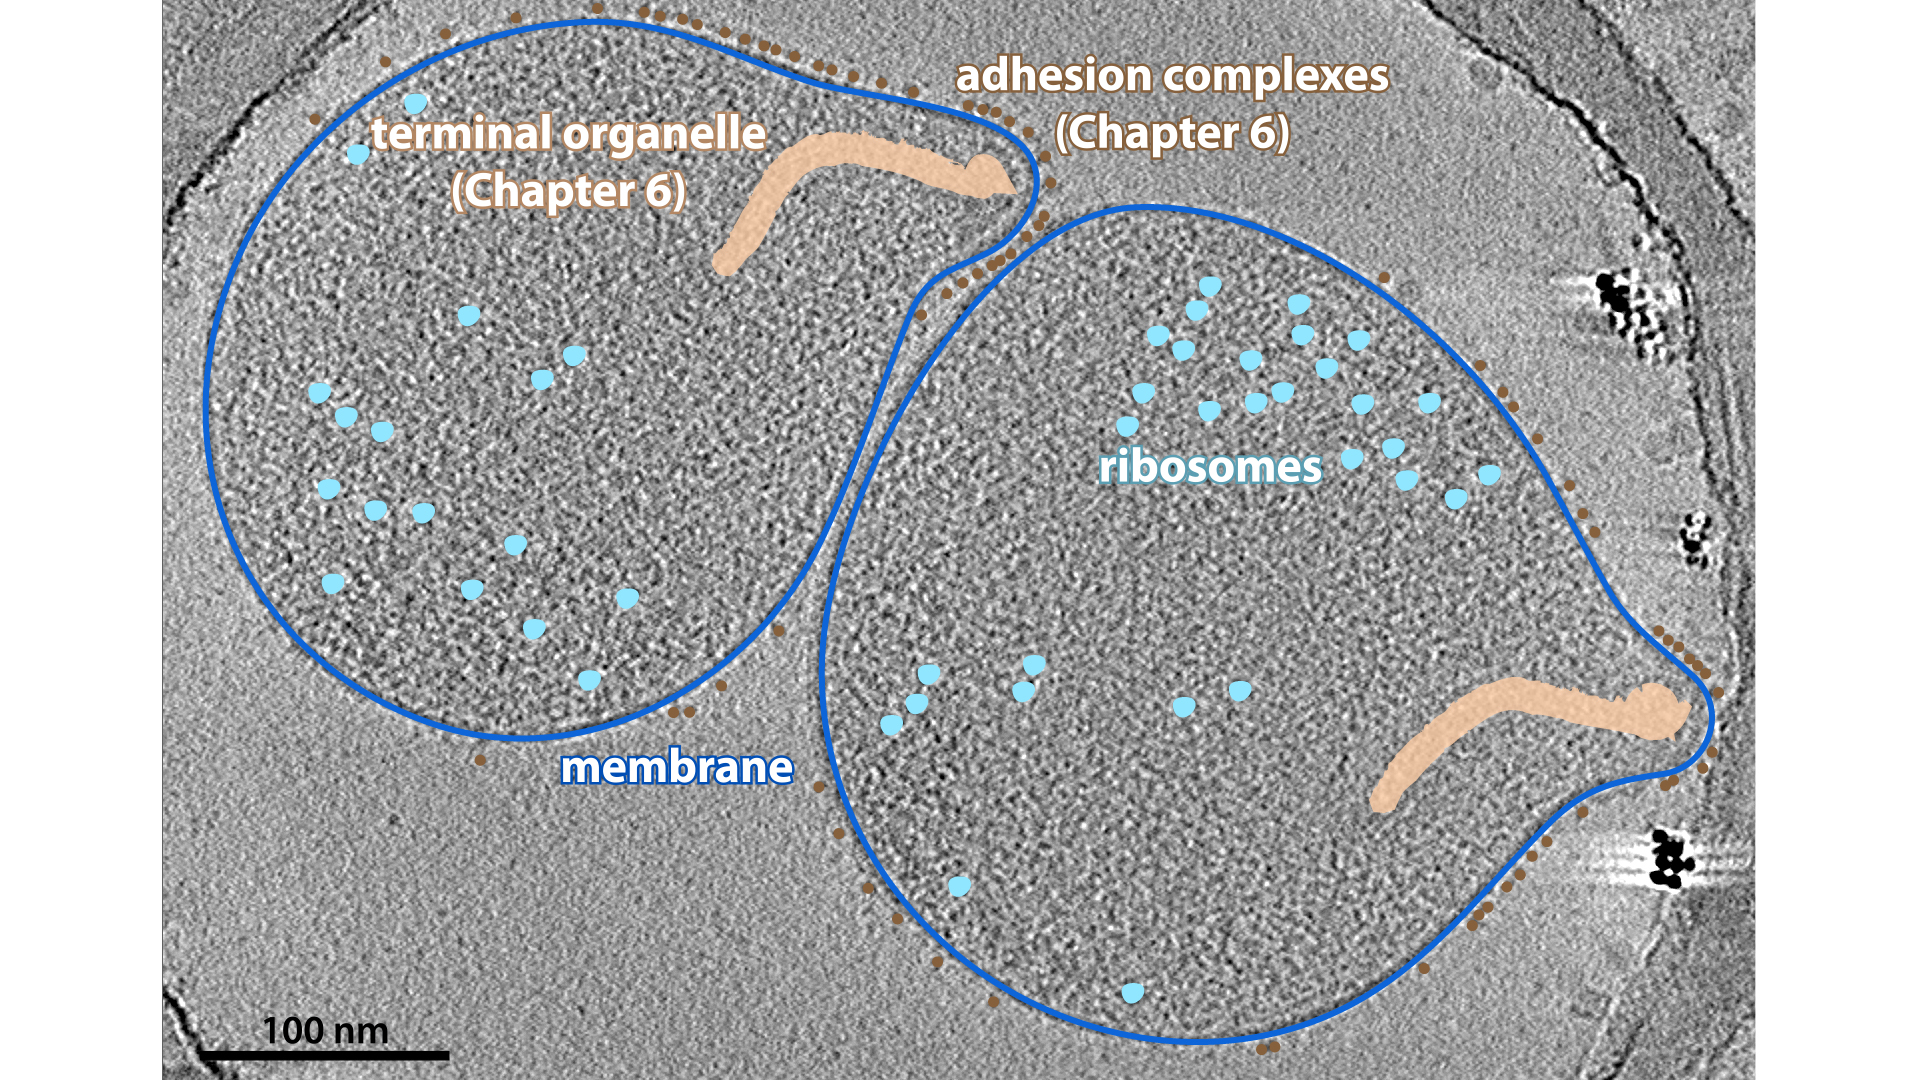
\includegraphics{img/02_static/2_1_Mgenitalium}

\begin{figure}
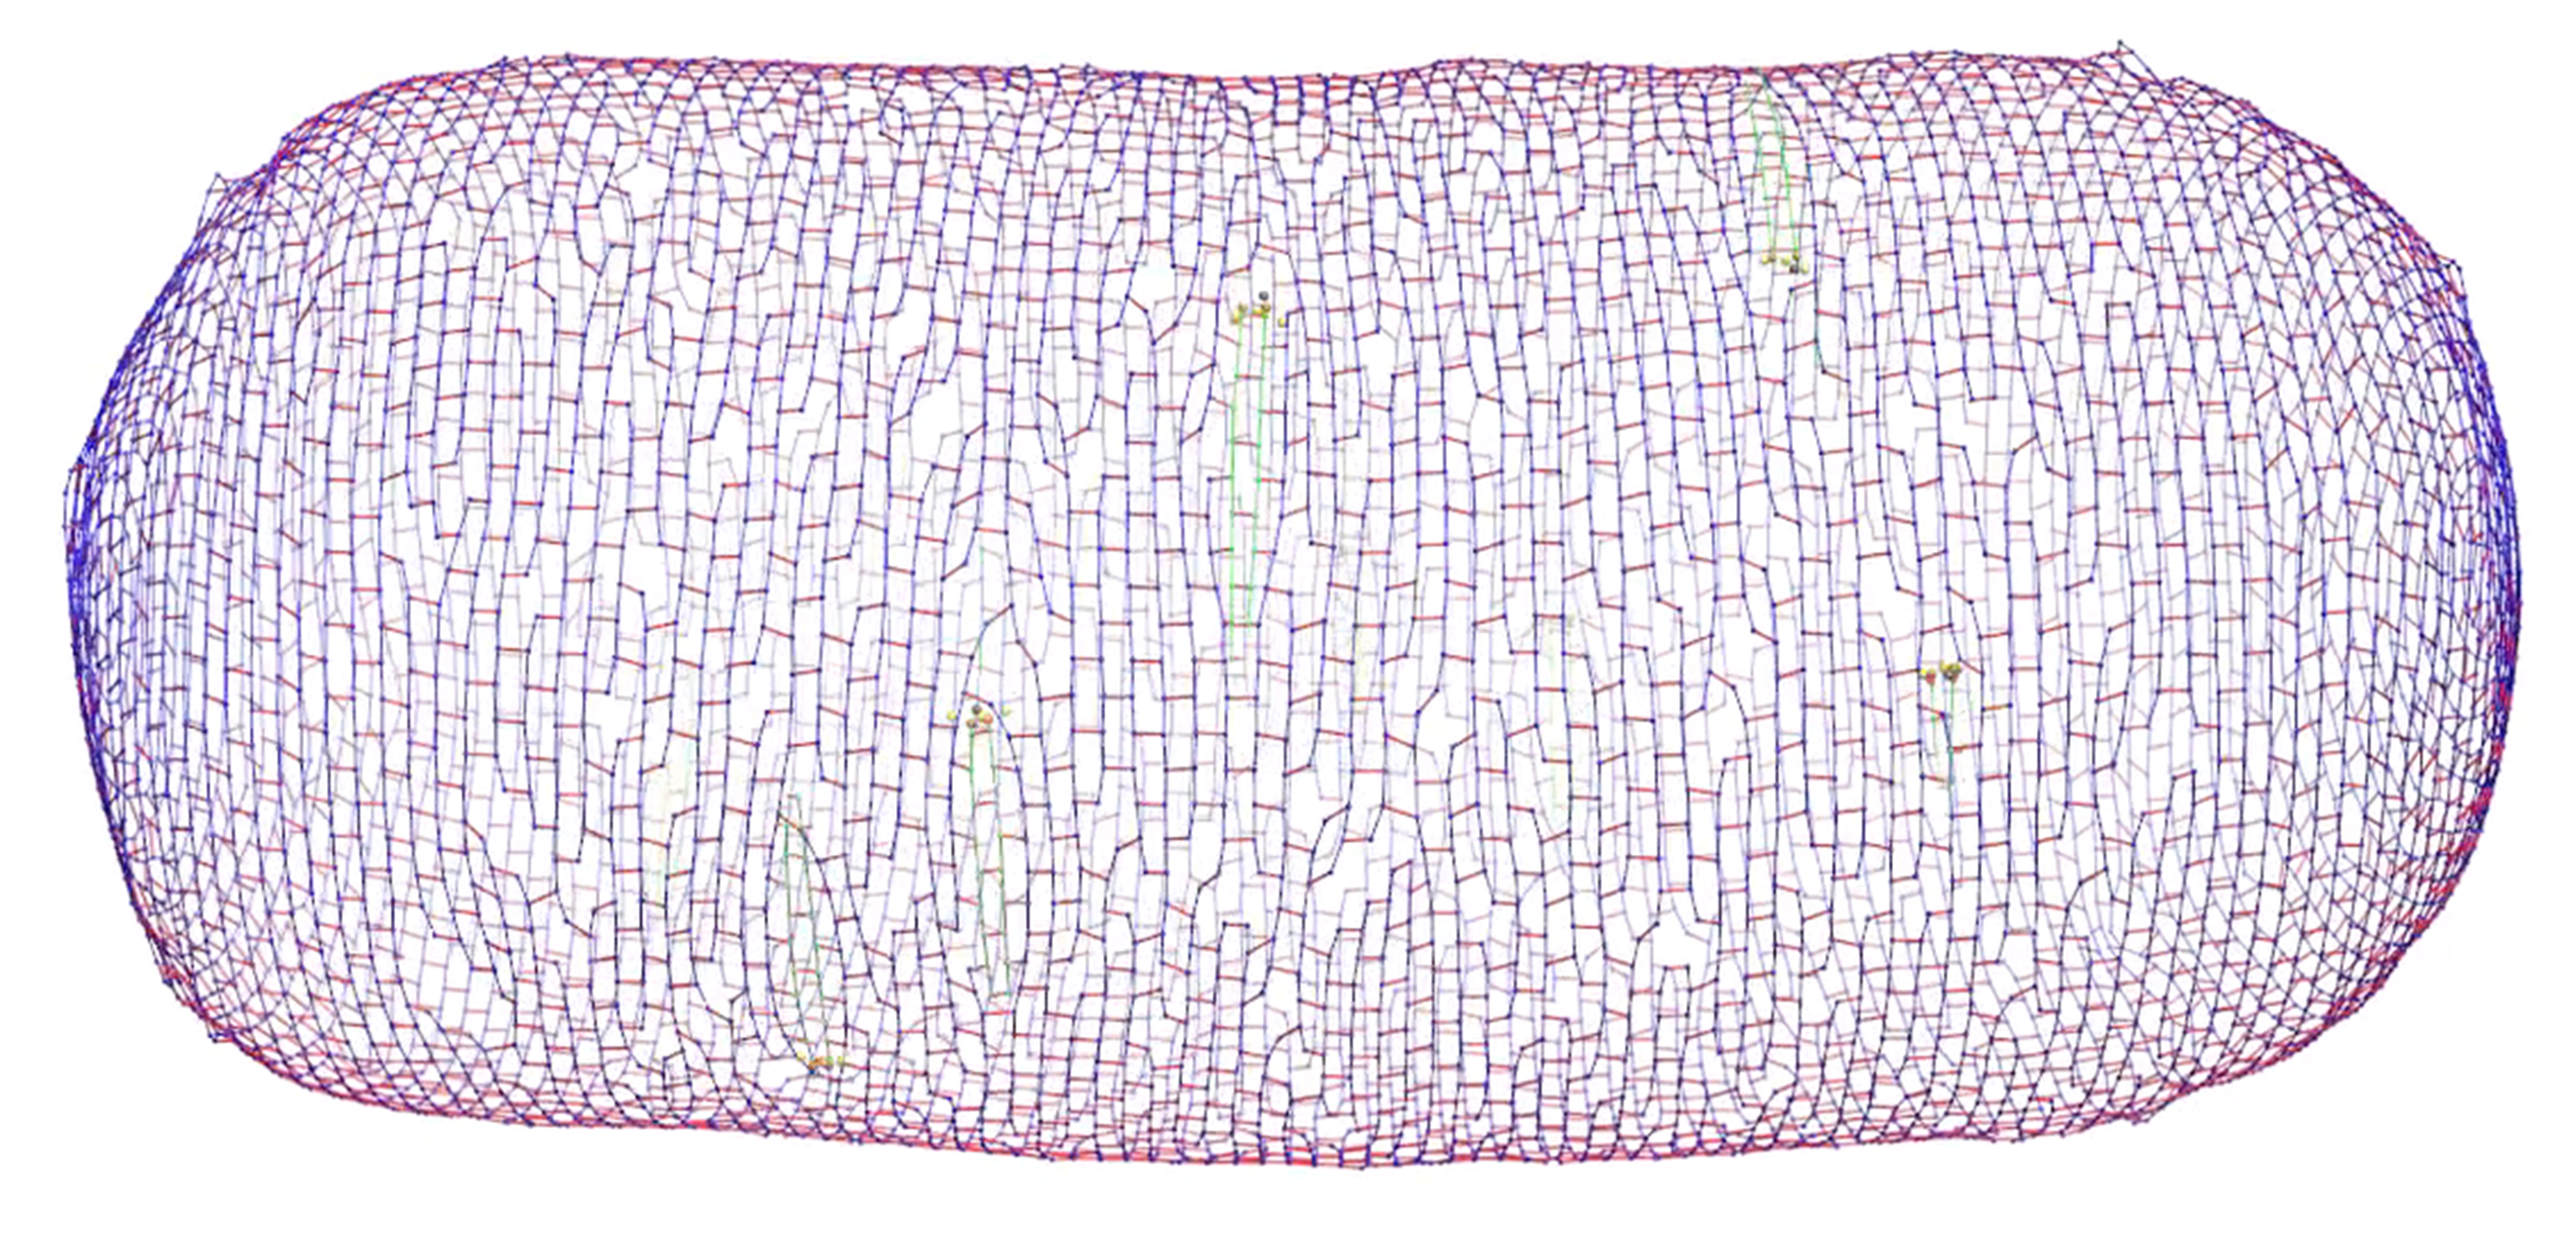
\includegraphics{img/02_schematic/2_3_2_SacculusRemodeling} \caption[Sacculus remodeling]{Sacculus remodeling}\label{fig:2-3-2}
\end{figure}

Encasing your cell in a rigid scaffold presents a problem: how can it
grow? It's easy to make membranes larger simply by adding more lipids.
But to add more peptidoglycan strands, they have to be linked into the
existing network, which means breaking existing links to accommodate
them. In fact, cells remodel their sacculi with the tools you'd expect:
an enzyme that links glycan sugars into strands, an enzyme that links
strands together with peptide bonds, and an enzyme that cuts these
peptide links. Remember, though, that your cell, with its solute-rich
interior, has a turgor pressure pushing outward with a force of maybe 3
atmospheres, equivalent to what we would feel at a depth of 20 meters in
the ocean. This is more than enough to lyse an exposed bacterial
membrane. So these tools must be used carefully to ensure that the cell
doesn't burst. We're still figuring out exactly how this works, with
help from computer simulations like this one. Here you see a model of an
Escherichia coli sacculus being enlarged using the three enzyme tools we
just described. This simulation was run to test whether just having the
tools function in a complex rather than separately might give enough
coordination for smooth, safe growth. (The answer was yes.)

More: Diderm archaea Nearly all diderm cells are bacteria. Not all,
though. As you see here, Ignicoccus hospitalis, an archaeon, has an
outer membrane that appears very loosely associated with the cell,
forming an extra large periplasm. You can see membrane-bound vesicles
shuttling cargo across this vast space (more about vesicles on the next
page). Interestingly, this is also an exception to the rule that the
inner membrane of diderms is ``energized'' (proton-tight). In I.
hospitalis, it is the outer membrane that contains the ATP synthases.
These unusual characteristics suggest a symbiotic origin for this
species; perhaps its ancestor used to live inside a host cell, which was
eventually reduced to a mere membrane.

\section{Borrelia burgdorferi}\label{borrelia-burgdorferi}

What else can you do with an extra membrane? Since membranes make
excellent containers for molecules, why not get into the shipping
business? In the coming chapters (especially Chapter 8), you'll see some
of the ways that cells interact with each other and their environment.
For diderm bacteria, many of these interactions are made possible by
outer membrane vesicles (``little bladders'')--self-contained pockets
budded off the membrane. The vesicles may carry cargo of antibiotics to
inhibit competitors' growth, or toxins to lyse neighboring cells. Or
enzymes to digest those lysed remains into nutrients that your cell can
easily take up as food. Alternatively, they may carry emergency kits
(first aid and survival factors) for other members of a community
biofilm. The appearance of these vesicles varies as much as their
contents \protect\hyperlink{Vesicle_morphologies}{More: Vesicle
morphologies}. They are usually spherical, of a consistent size, and
often come off the cell at one or a few sites, forming chains, as you
can see in this Borrelia burgdorferi cell.

Not all diderms produce outer membrane vesicles, and even for the ones
that do, we still don't know exactly how they do it. Maybe it happens
spontaneously due to the physics of lipids and proteins in a certain
configuration. Or maybe there's a dedicated protein machine in the
membrane, blowing bubbles. Some archaea (monoderms) also produce
membrane vesicles. They're less studied than their bacterial
counterparts, but likely serve similar roles in metabolism and community
interactions.

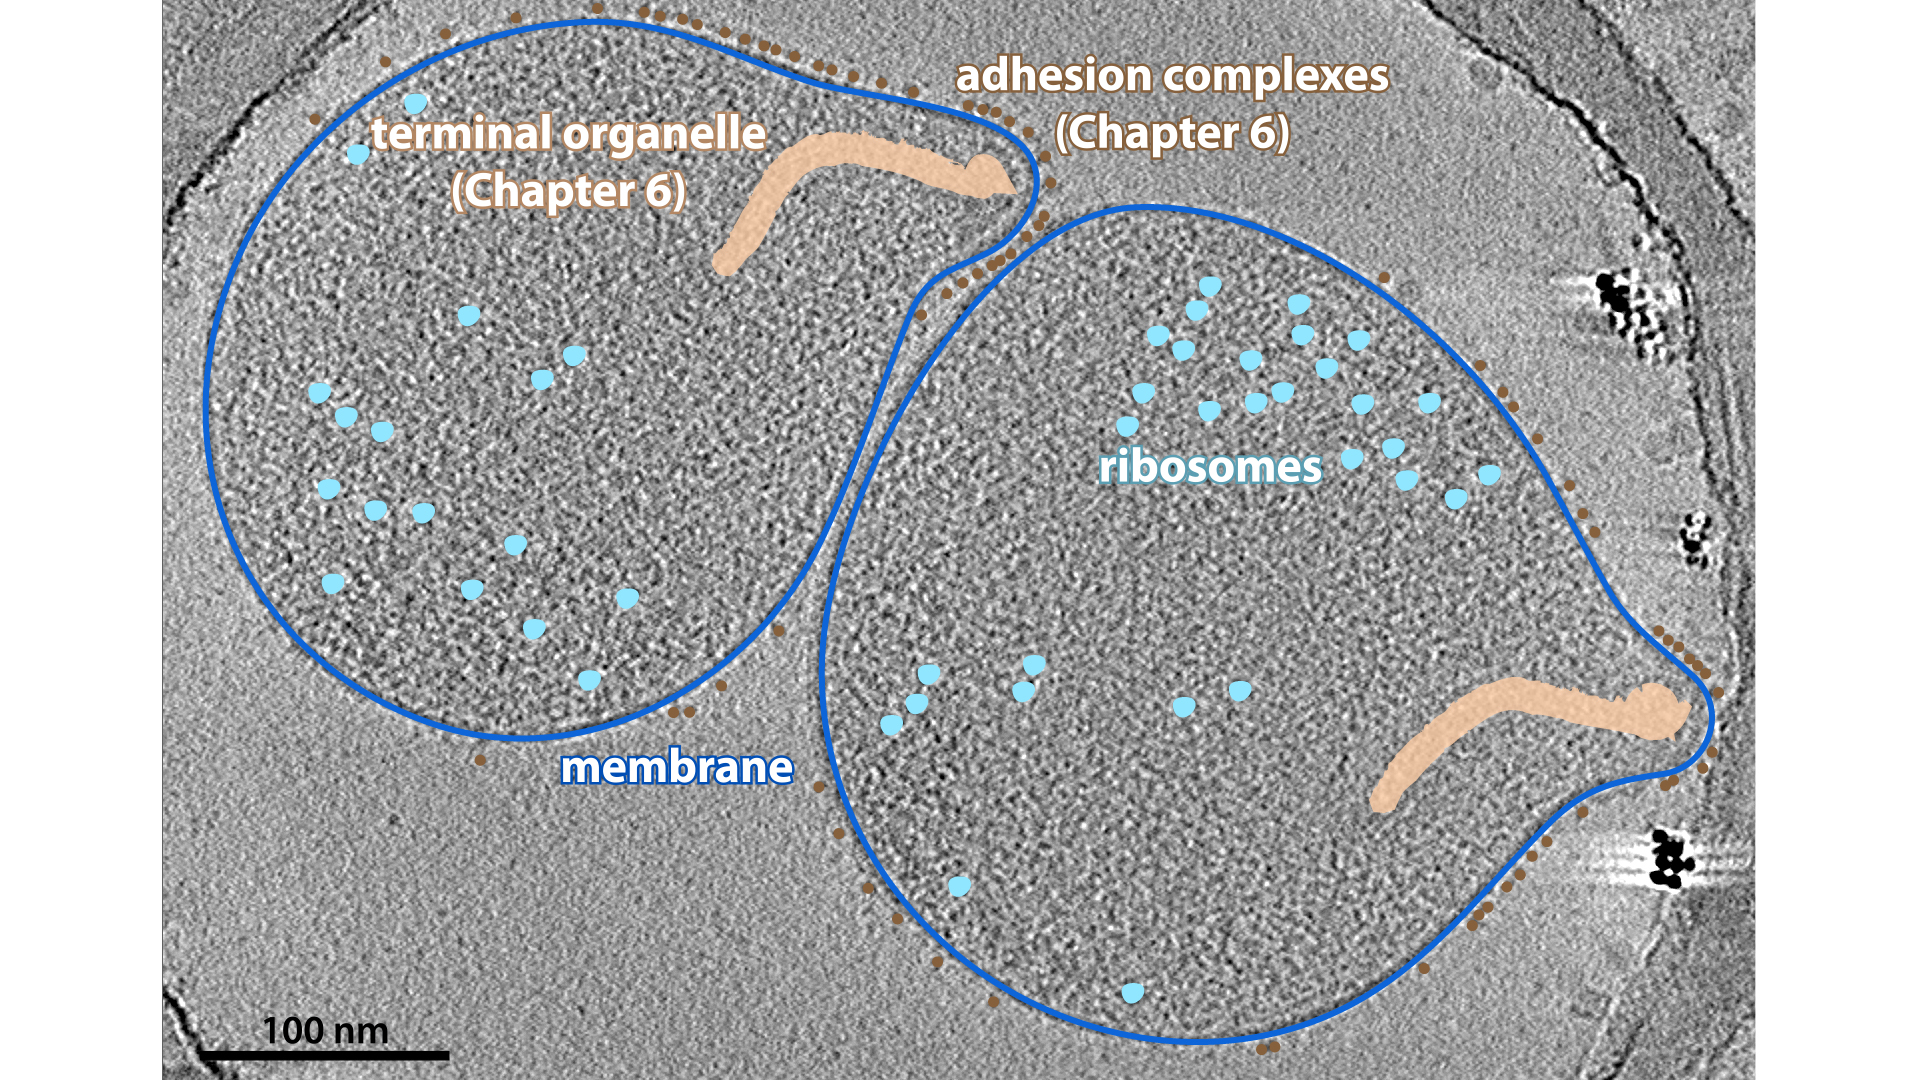
\includegraphics{img/02_static/2_1_Mgenitalium}

\hypertarget{Vesicle_morphologies}{\subsection{Borrelia
burgdorferi}\label{Vesicle_morphologies}}

Different species can produce outer membrane vesicles that look very
different. The same species can also produce vesicles that look very
different. Sometimes they come off the cell as a chain of spheres;
sometimes the spheres remain connected, like a string of pearls;
sometimes vesicles form long tubes instead, like from this Borrelia
burgdorferi cell. Sometimes the same chain can be tubular in one section
(usually at the base, connected to the cell), and a string of spheres in
another.

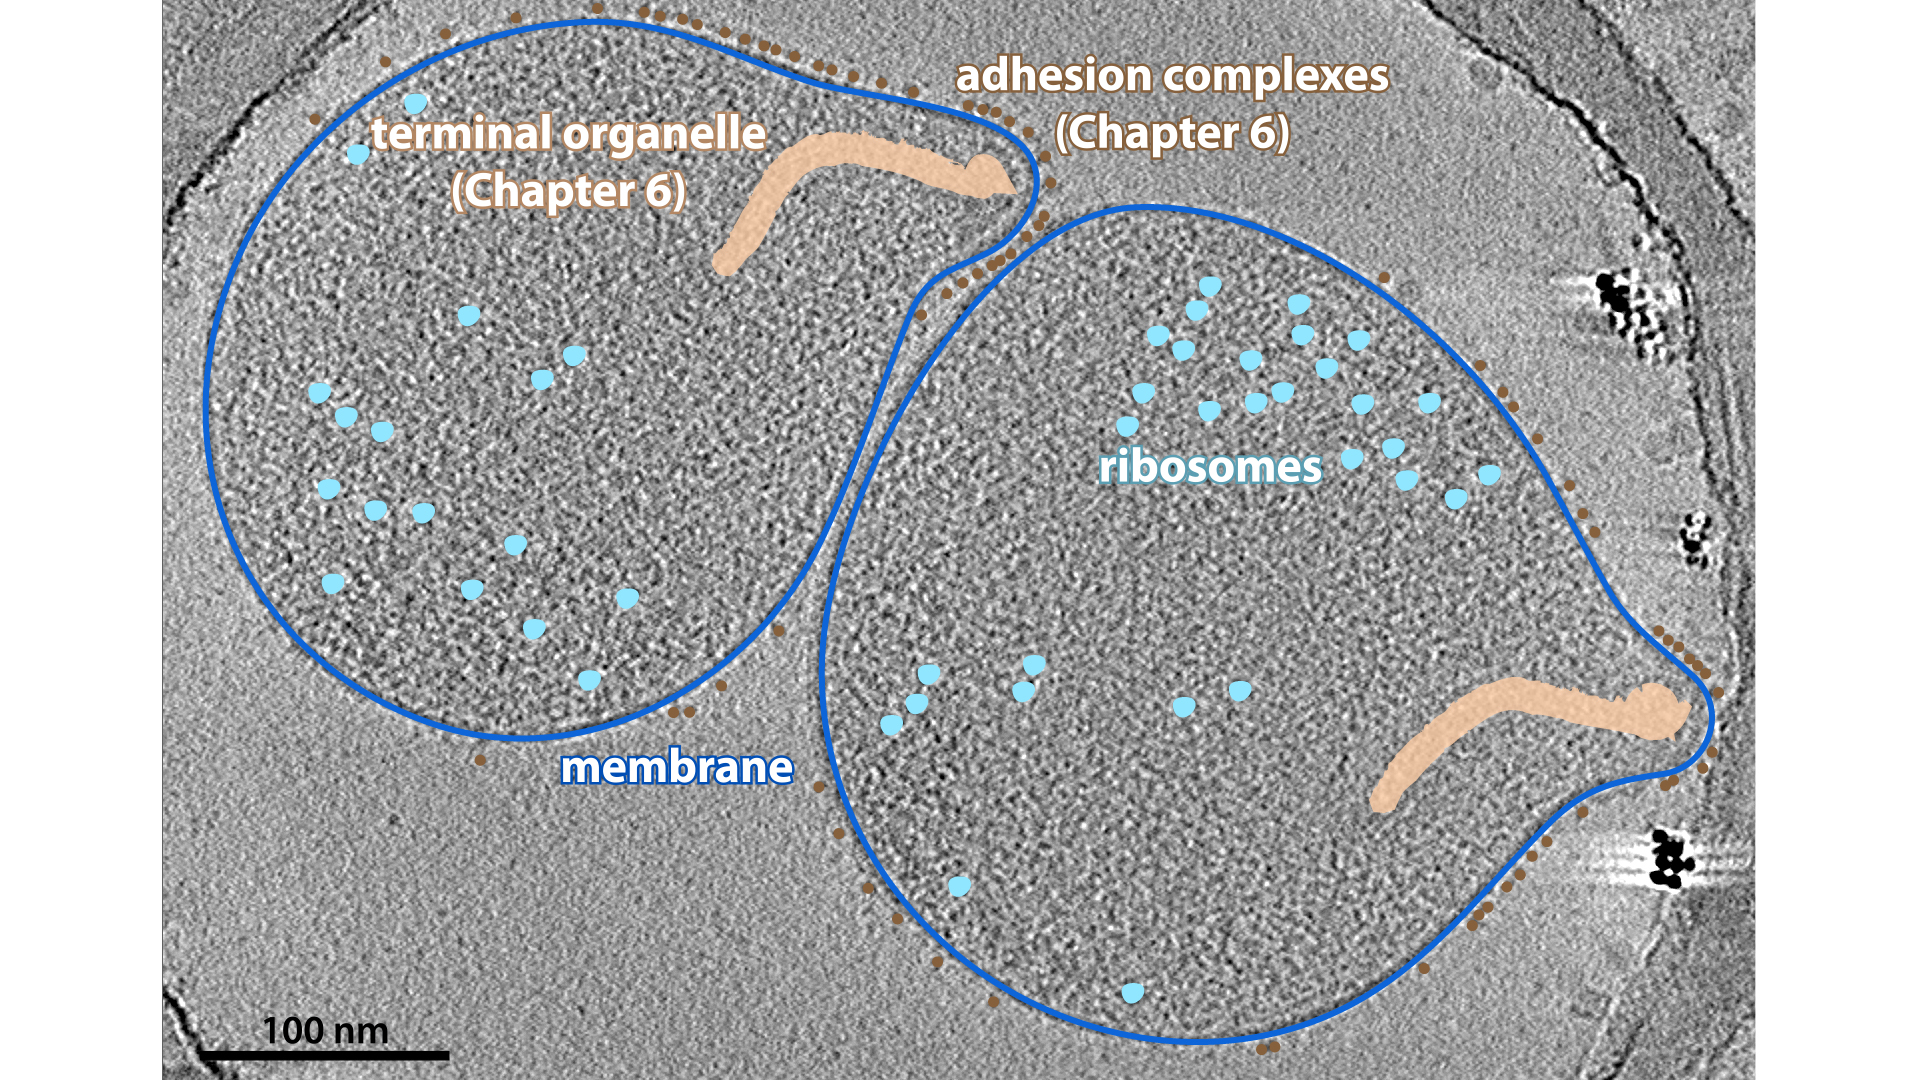
\includegraphics{img/02_static/2_1_Mgenitalium}

\subsection{Myxococcus xanthus}\label{Inner_membrane_vesicles}

Not all vesicles come from the outer membrane. The cytoplasmic or inner
membrane can also form vesicles that are released into the cytoplasm, as
in this Myxococcus xanthus cell, or into the periplasm. This seems to be
a less regulated process than outer membrane vesicle formation, and we
see it in many species when they are stressed by low nutrients or high
cell density, suggesting that it is a general phenomenon. Cells shrink
in harsh conditions (more on that in Chapter 7), so cytoplasmic or
periplasmic vesicles may simply offer a place to put the extra membrane
or, more optimistically, to store it until the time comes to grow again.
Just as with outer membrane vesicles, the appearance of cytoplasmic
vesicles can vary widely
\protect\hyperlink{Cytoplasmic_vesicle_variety}{More: Cytoplasmic
vesicle variety}.

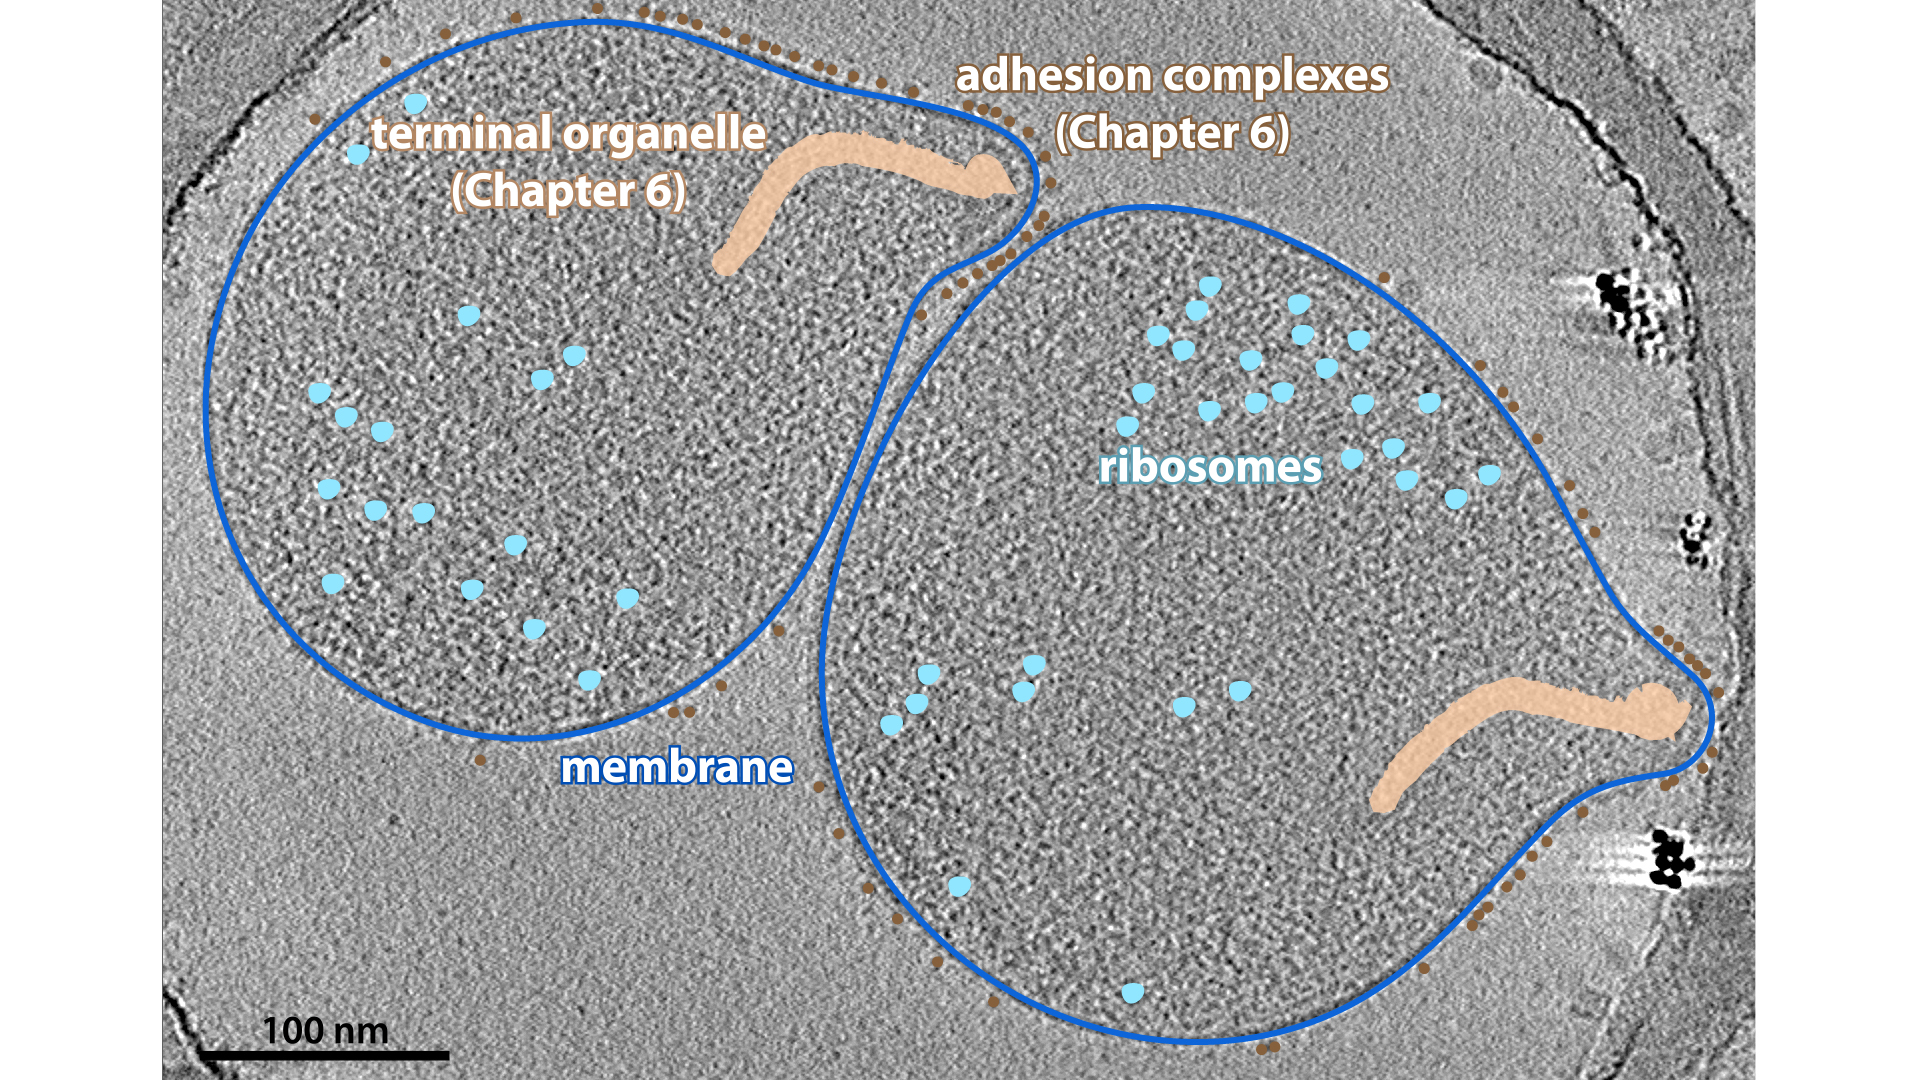
\includegraphics{img/02_static/2_1_Mgenitalium}

\hypertarget{Cytoplasmic_vesicle_variety}{\subsection{Prosthecobacter
debontii}\label{Cytoplasmic_vesicle_variety}}

Cytoplasmic vesicles exhibit a variety of sizes and shapes. Some are
nested, with vesicles inside vesicles. In this Prosthecobacter debontii
cell, you can see two other morphologies. One is a large, flattened
horseshoe-shaped vesicle. Another is a more typical spherical shape, but
is decorated with what looks like protein complexes.

This cell also has unusual structures on its surface that have yet to be
identified.

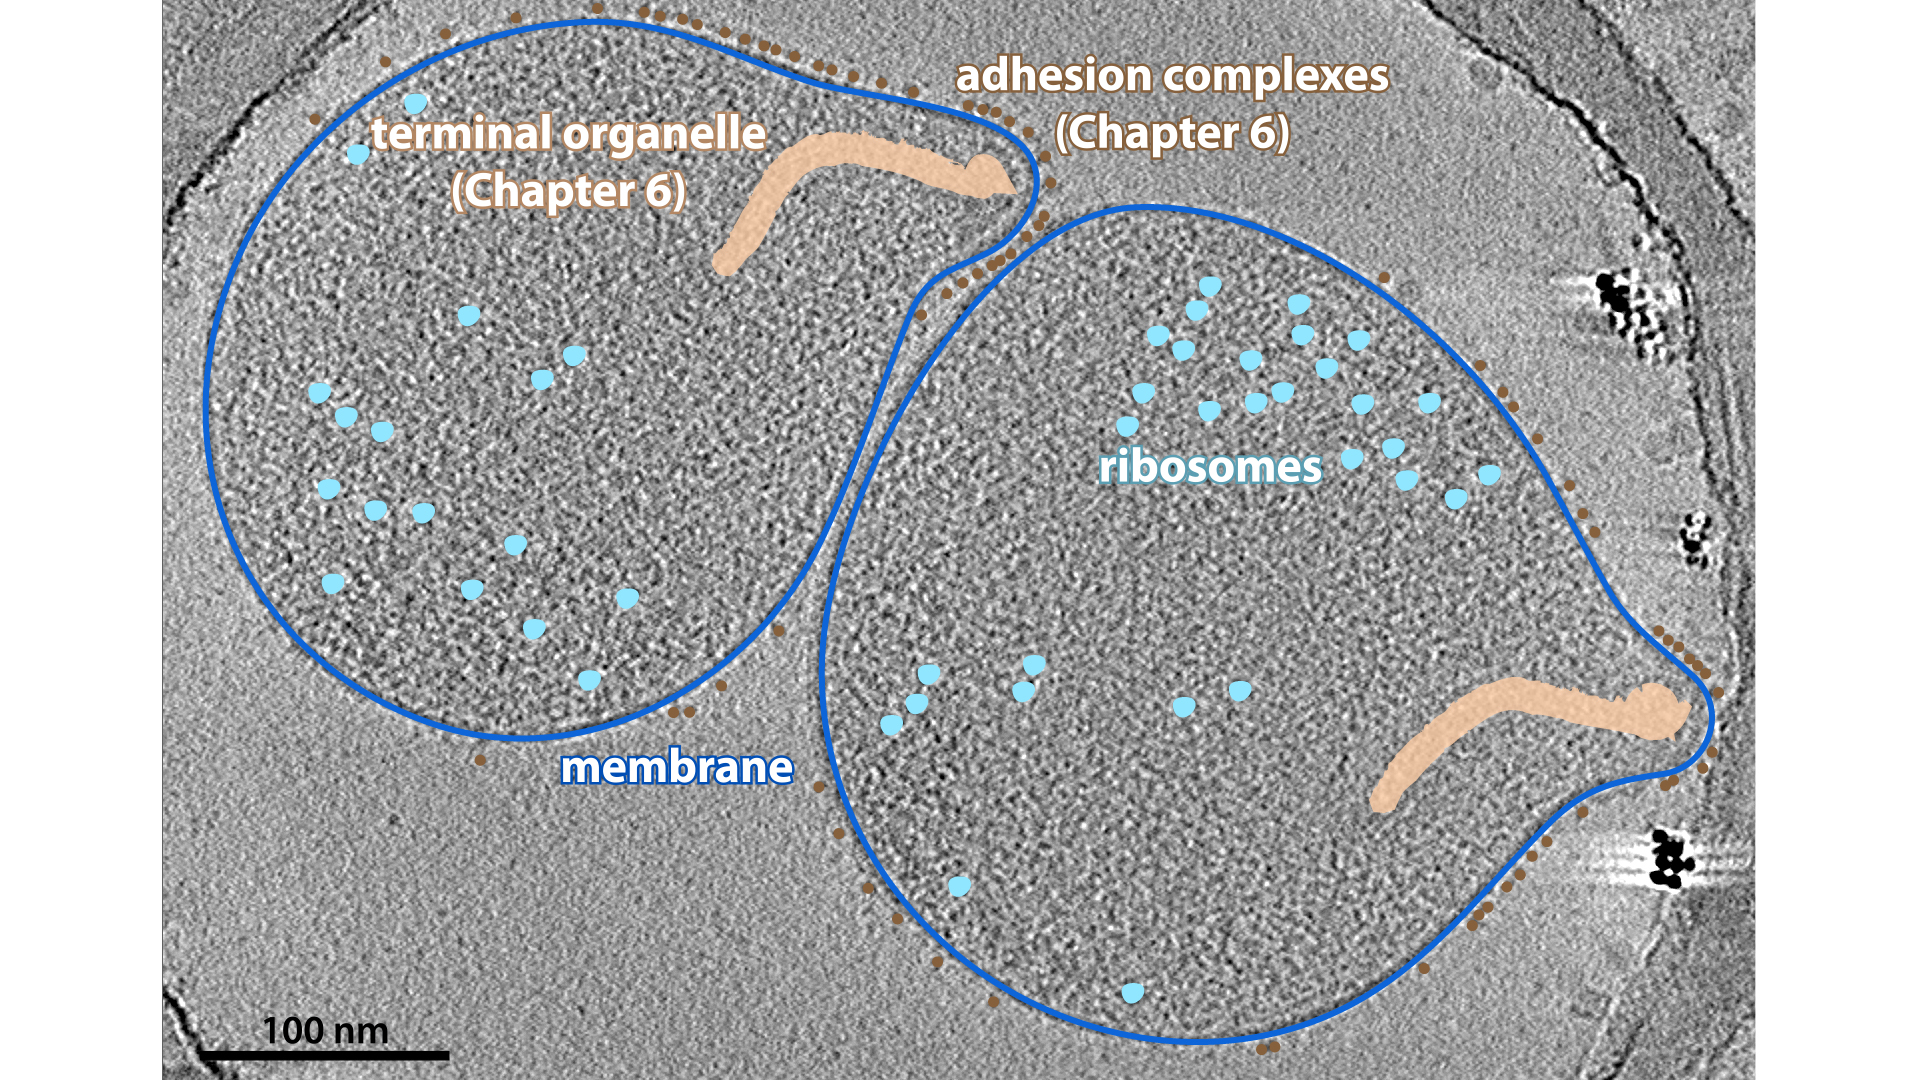
\includegraphics{img/02_static/2_1_Mgenitalium}

\section{Mycoplasma marinum}\label{mycoplasma-marinum}

Evolution is endlessly creative, providing exceptions to nearly every
classification rule. We've just described a neat breakdown of bacteria
into monoderms (one membrane, thick sacculus, positive Gram stain) and
diderms (two membranes, thin sacculus, negative Gram stain). But some
cells, like this Mycobacterium marinum, defy classification.
Mycobacteria are diderm, with an inner and an outer membrane, and a cell
wall. But they have unique molecules (named mycolic acids in their
honor) in the outer membrane. These acids interfere with Gram staining,
yielding an intermediate result between positive and negative. And their
sacculus consists of three layers, each with a unique molecular
composition \protect\hyperlink{fig:2-5-1}{Schematic -- Mycobacterial
architecture}. In this case, the middle layer is the familiar
peptidoglycan.

When you look at the schematic, you'll see another layer outside the
outer membrane. This layer, the capsule, isn't visible in the movie of
the cell, though. It is made up of ``Extracellular Polymeric
Substance,'' abbreviated EPS, or long chains of sugars, sometimes linked
to the outer membrane and sometimes free-floating. These sugars don't
interact strongly with electrons, so the capsule is usually invisible by
electron microscopy. But in fact, many bacteria (mostly diderm, but also
some monoderm) have a capsule. The capsule can help bacteria attach onto
surfaces and offers an extra layer of protection, trapping water to
prevent desiccation and making it more difficult for hydrophobic
molecules like detergents to get through to disrupt the membranes. It
also makes it more difficult for viruses to reach the cell, and for
eukaryotic ``predators'' like macrophages to eat it.

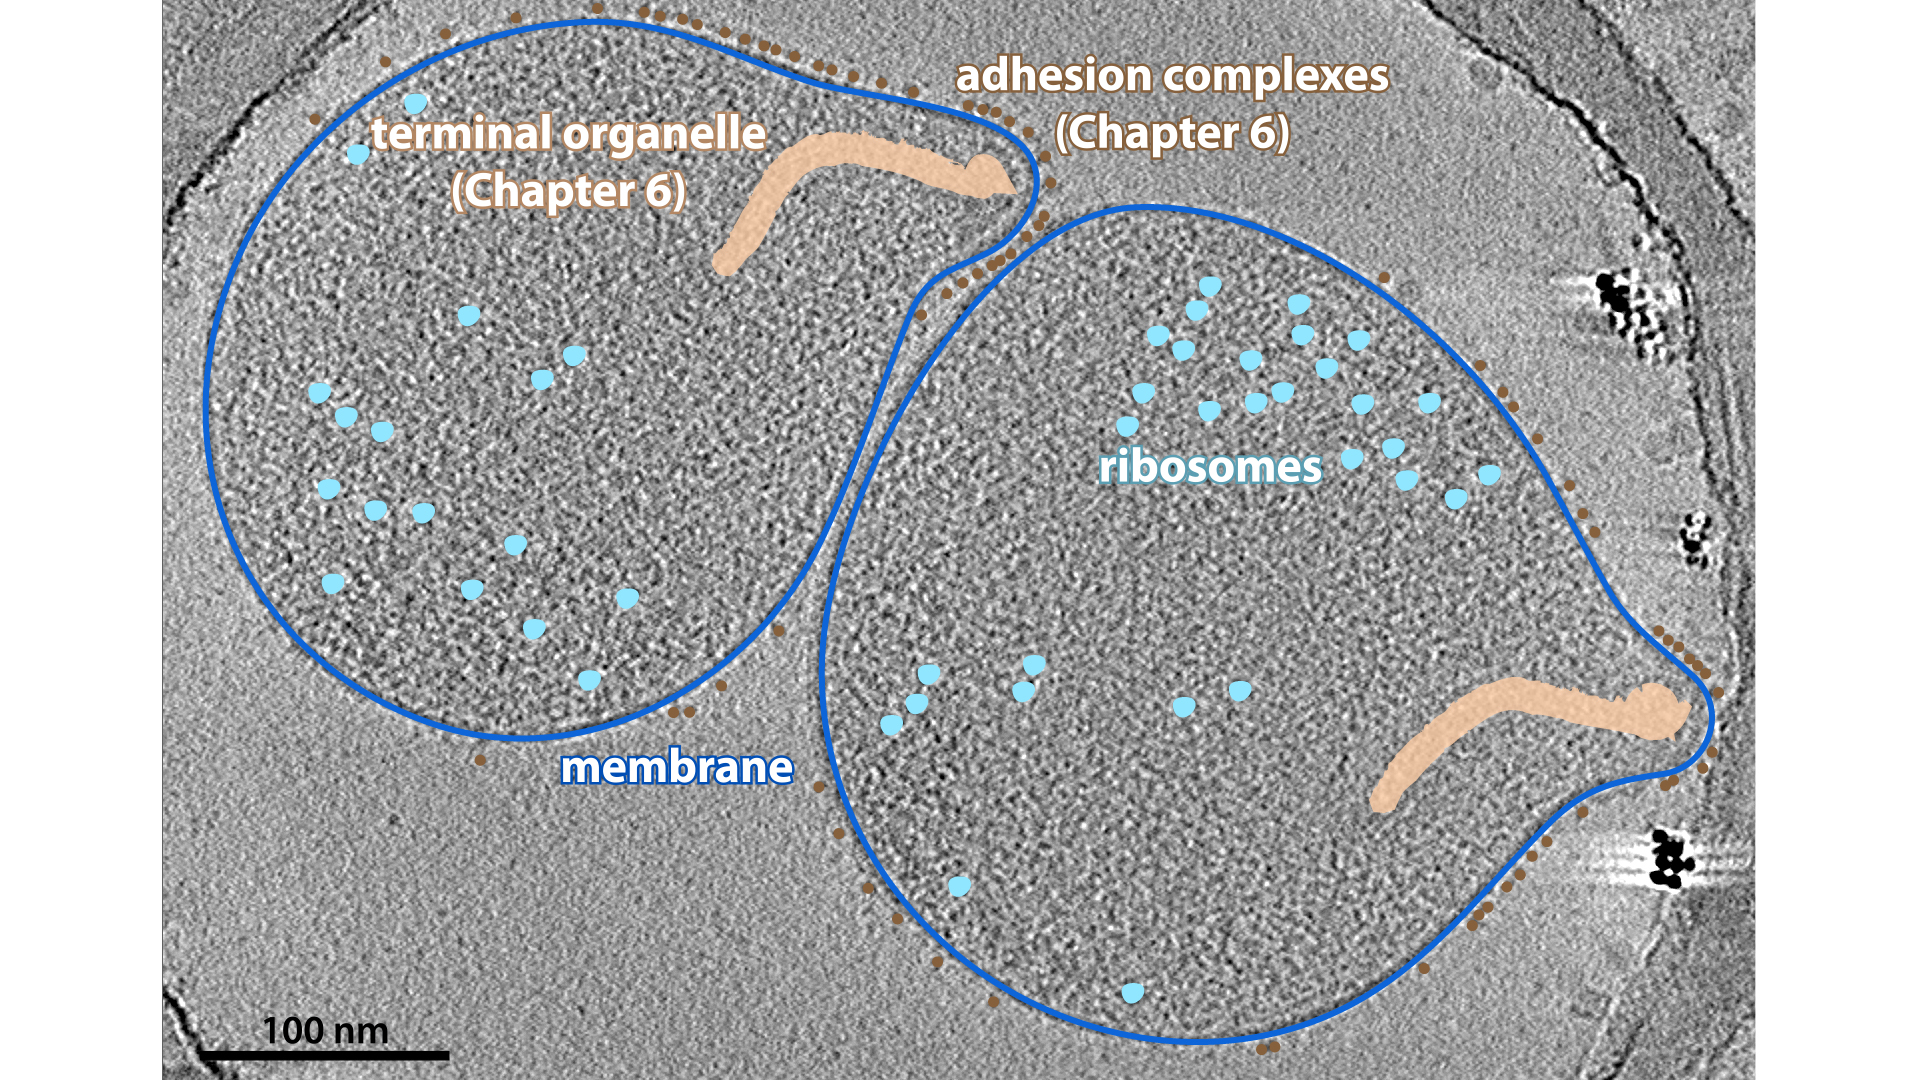
\includegraphics{img/02_static/2_1_Mgenitalium}

\begin{figure}
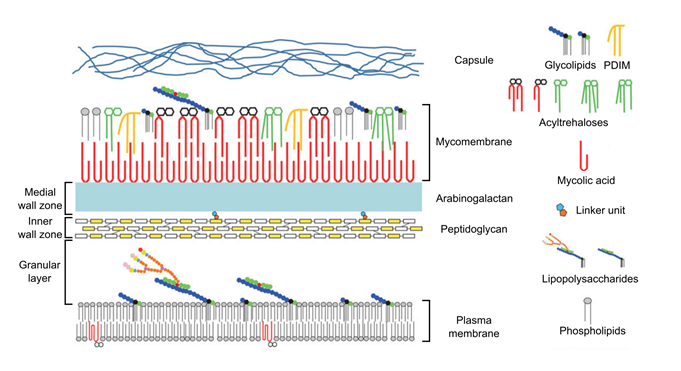
\includegraphics{img/02_schematic/2_5_1_Mycobacteria} \caption[Mycobacterial architecture]{Mycobacterial architecture}\label{fig:2-5-1}
\end{figure}

A unique architecture encloses Mycobacterial cells. Note the outer
membrane, with lipids only in the outer leaflet, and mycolic acids
forming the inner. Note also the multiple strata of sugars in the cell
wall. Also note the capsule depicted outside the outer membrane.

\section{Caulobacter crescentus}\label{caulobacter-crescentus}

How else can you protect your cell from the rigors of a harsh world?
What about encasing it in an armored shell a la the armadillo? Many
bacteria (both monoderms and diderms) and archaea use modular proteins
for this purpose, interlocking Lego-block-like pieces into a shell
called the Surface Layer, or S-layer. You can guess that this must offer
a significant evolutionary advantage since up to 15\% of the total
protein in the cell can be found in the structure. In fact, S-layers
play many roles for cells, some of which you'll see on the next page,
but one of their main functions is as a gatekeeper, preventing large
things like viruses from reaching the membrane.

S-layers are crystalline lattices, and they can be striking in
appearance, as on this Caulobacter crescentus cell. Amazingly, the
lattice is made from (many copies of) a single protein
\protect\hyperlink{fig:2-6-1}{Schematic -- S-layer architecture}. The
pinwheel-like subunits interact laterally, leaving pores large enough
for nutrients to pass through, but not large enough for viruses. The
modular nature of the lattice means that units can be popped in as the
cell grows, or popped out to allow a cell appendage to poke through. In
general, S-layers are quite accommodating; they don't even interfere
with the production of outer membrane vesicles
\protect\hyperlink{Nanopods}{More: Nanopods}. S-layer proteins can also
be modified to alter their properties; for instance attachment of a
sugar can enable them to stick the cell to a surface.

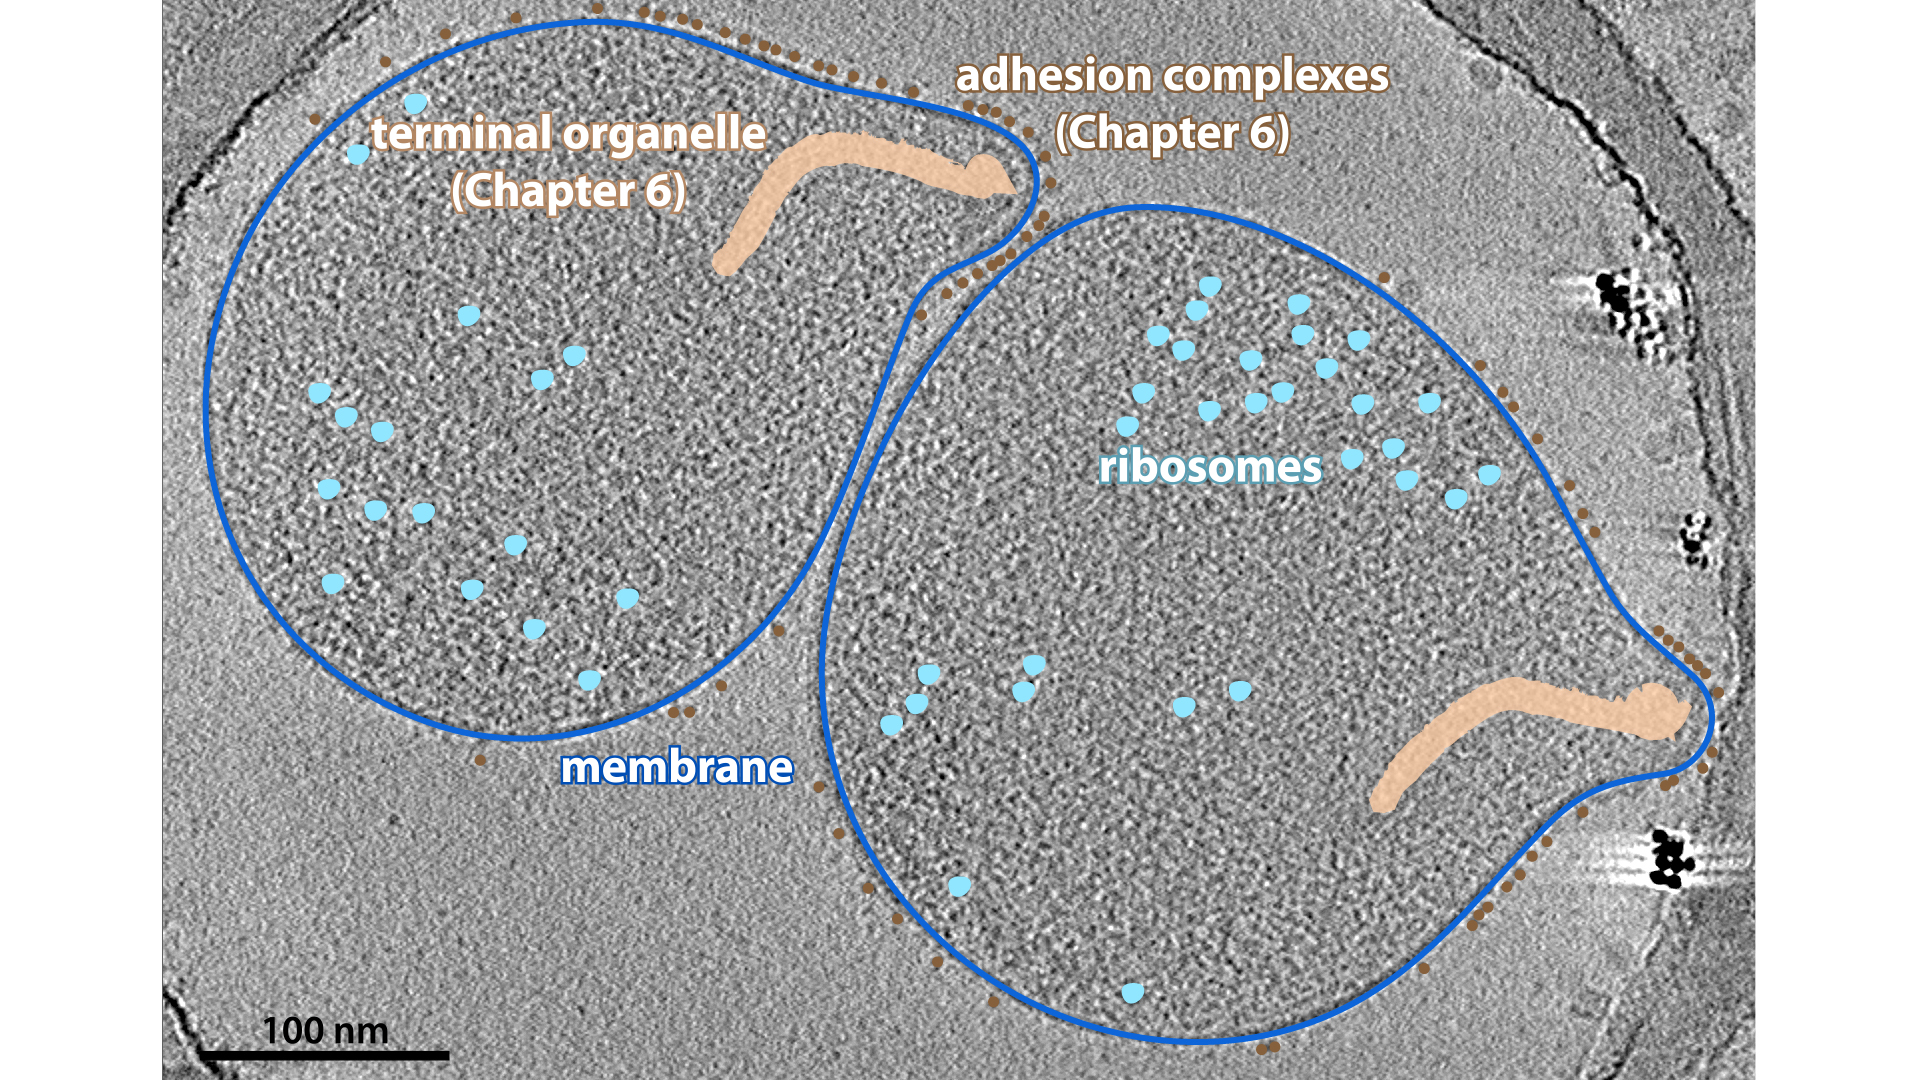
\includegraphics{img/02_static/2_1_Mgenitalium}

\begin{figure}
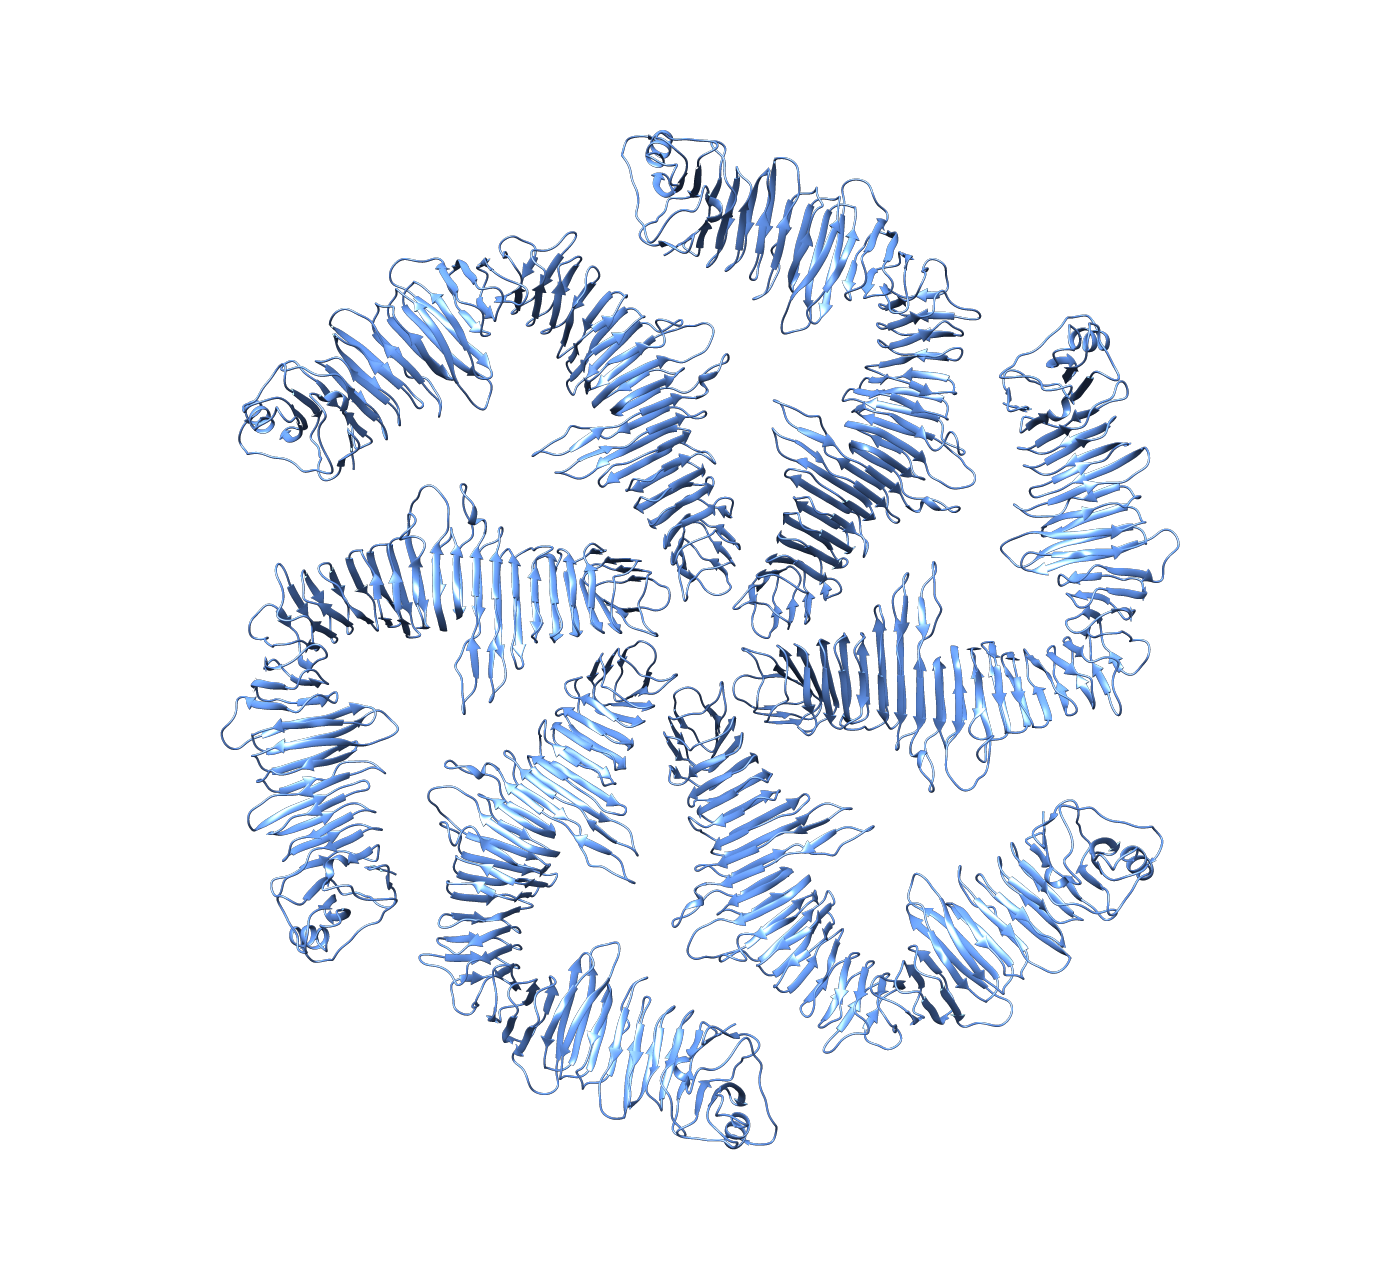
\includegraphics{img/02_schematic/2_6_1_SLayerTop} \caption[S-layer architecture]{S-layer architecture}\label{fig:2-6-1}
\end{figure}

A single protein forms the S-layer you just saw in Caulobacter
crescentus. The protein has two domains. The bottom domain anchors to
lipoproteins attached to the outer membrane. The top domain forms the
canopy of the S-layer, organizing hierarchically into hexameric rosettes
like this that in turn pack into a larger hexameric lattice. This
lattice is flexible enough to curve around even narrow regions of the
cell (more on this stalk in Chapter 3).

\hypertarget{Nanopods}{\subsection{Delftia acidovorans}\label{Nanopods}}

Archaea and diderm bacteria with S-layers produce characteristic outer
membrane vesicles: they bud off with the S-layer attached. Delftia
acidovorans, like this produce so-called nanopods: chains of outer
membrane vesicles ensheathed in S-layer.

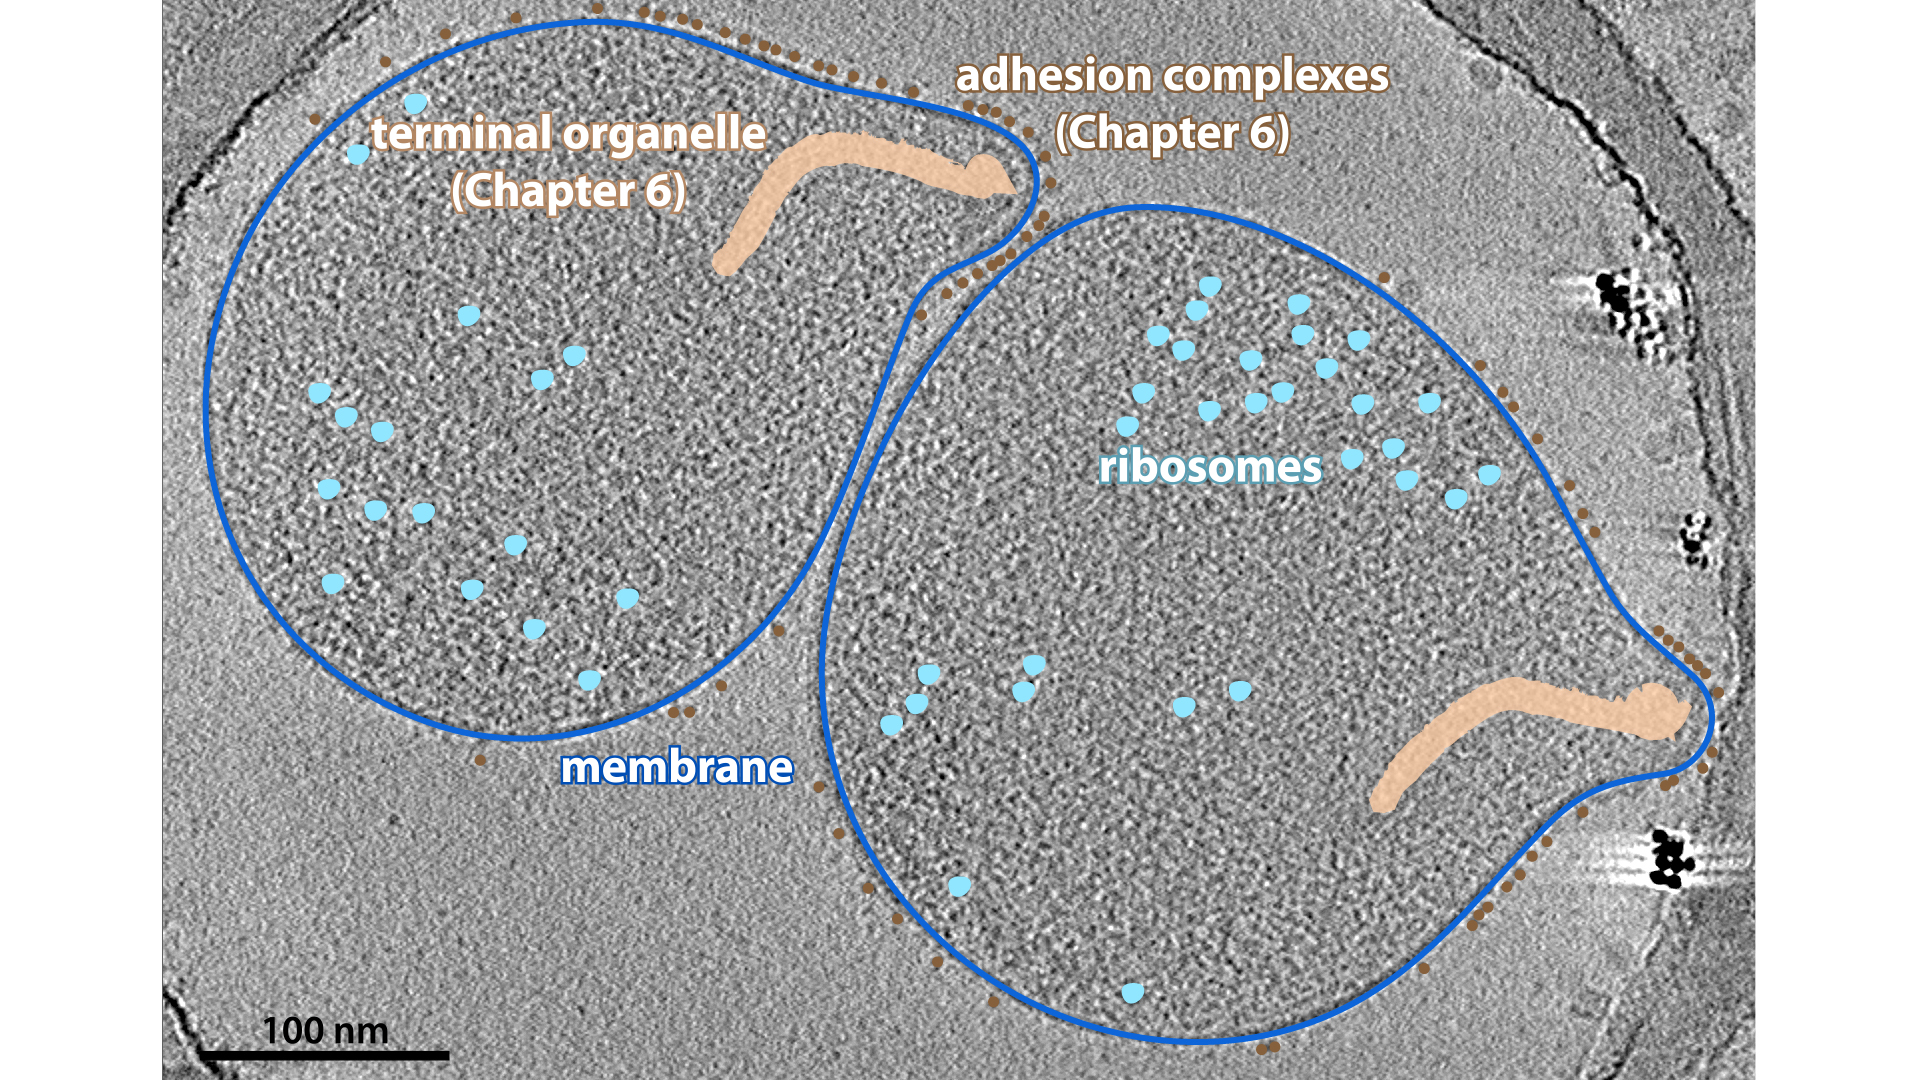
\includegraphics{img/02_static/2_1_Mgenitalium}

\section{Sulfolobus solfataricus}\label{sulfolobus-solfataricus}

One of the most striking features of the S-layer is how different it can
look in different species. For instance, compare this archaeal
Sulfolobus solfataricus cell to the bacterium on the last page, or to
other diderm \protect\hyperlink{M._alcaliphilum}{More: M. alcaliphilum}
or monoderm \protect\hyperlink{}{More: C. thermocellum} bacteria, or
archaea \protect\hyperlink{N._maritimus}{More: N. maritimus}
\protect\hyperlink{Methanoregula_formicica}{More: Methanoregula
formicica}. All S-layers are crystalline lattices of a single--or in a
few cases, two--proteins, but the particular pattern of the lattice
depends on the shape of this building block and how it multimerizes into
a higher-order structure. The shape of the building block varies
considerably; there is almost no sequence homology between S-layer
proteins from different species. And shapes come together in different
ways, forming repeating units of one, two, three (as on this cell),
four, or six blocks.

S-layers are very common in archaea like this cell. Most archaea don't
have cell walls, but the S-layer provides the same function of external
scaffolding. Remember, too, that nearly all archaea are monoderms,
lacking the extra periplasmic compartment that diderms have. Here again
the S-layer serves a similar function, enclosing a space around the
cell's membrane called the pseudo-periplasmic space. Just as with the
bacterial periplasm, this space serves as an antechamber for the cell,
restricting access by large molecules. In some cases, the
pseudo-periplasmic space also contains specific proteins that function
in metabolism.

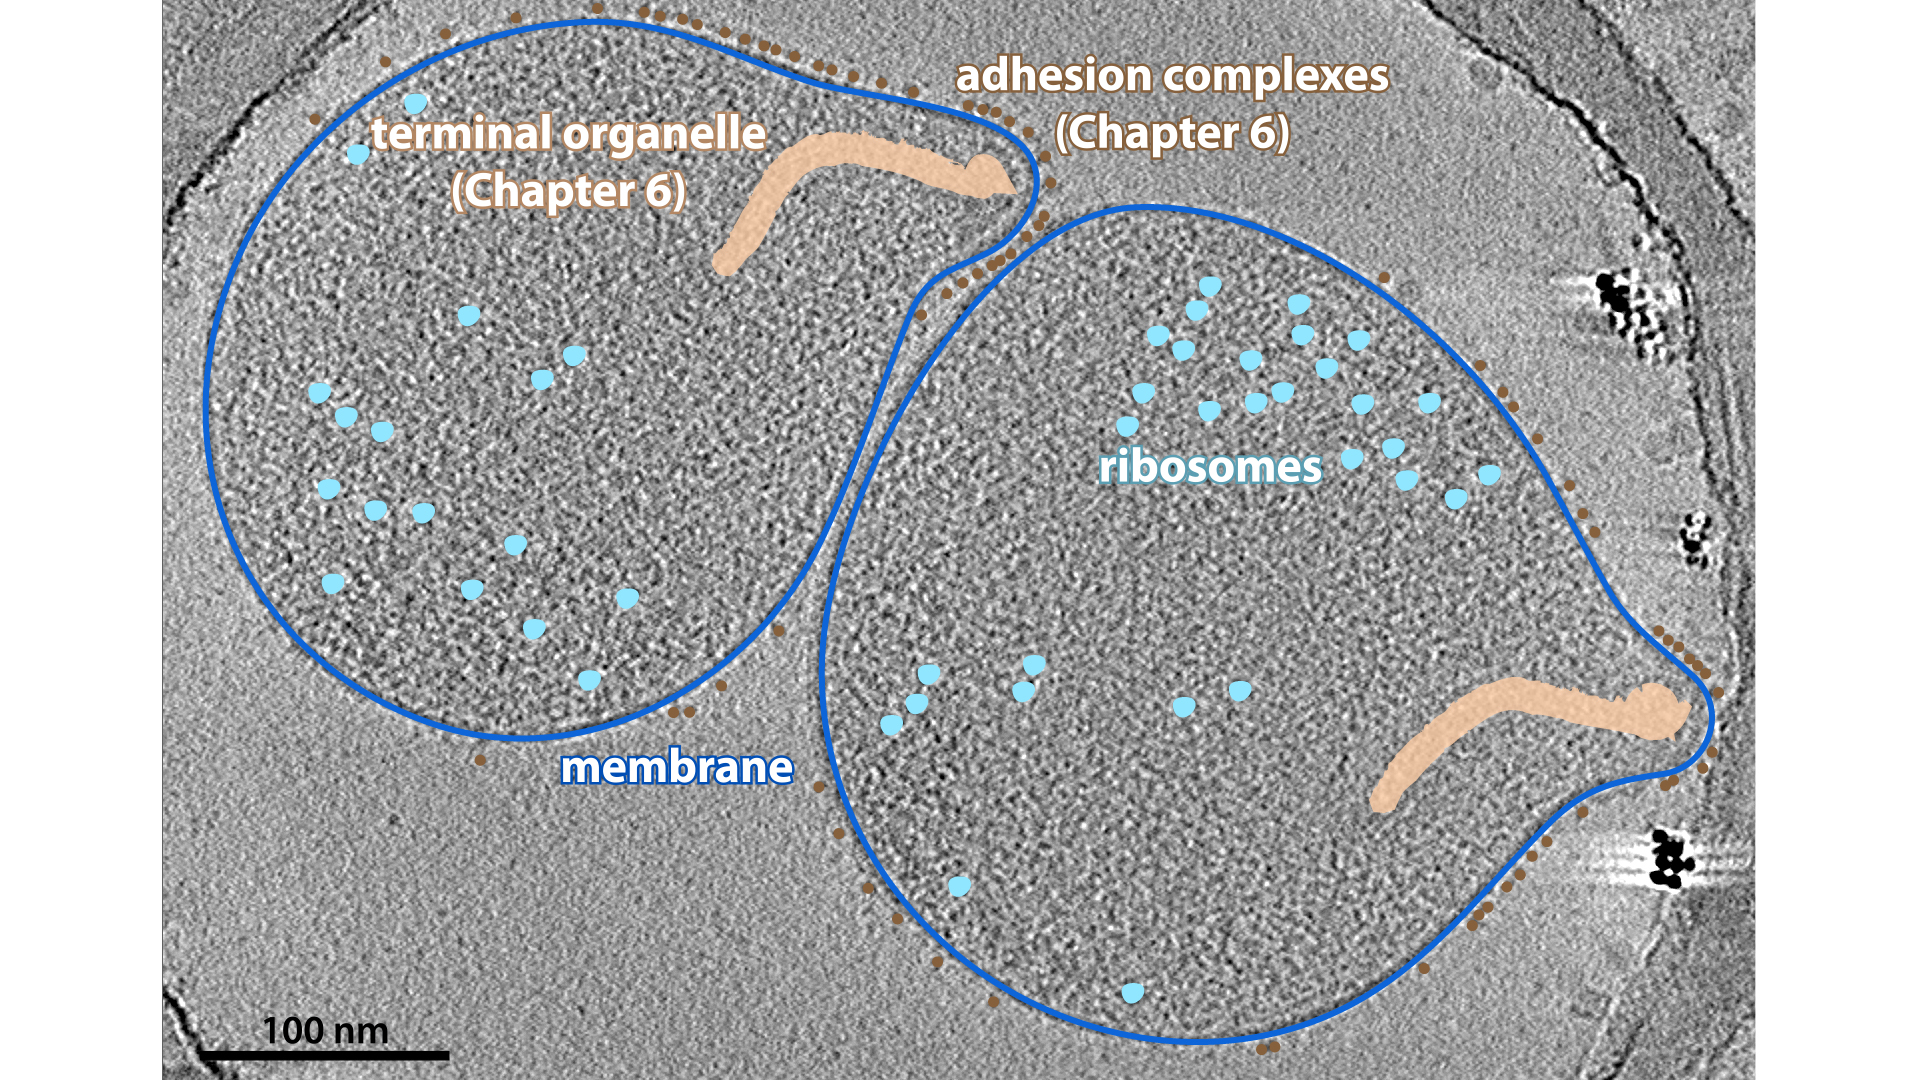
\includegraphics{img/02_static/2_1_Mgenitalium}

\hypertarget{M._alcaliphilum}{\subsection{Methylomicrobium
alcaliphilum}\label{M._alcaliphilum}}

In Methylomicrobium alcaliphilum, V-shaped S-layer proteins come
together to form cups that pack into a hexagonal pattern.

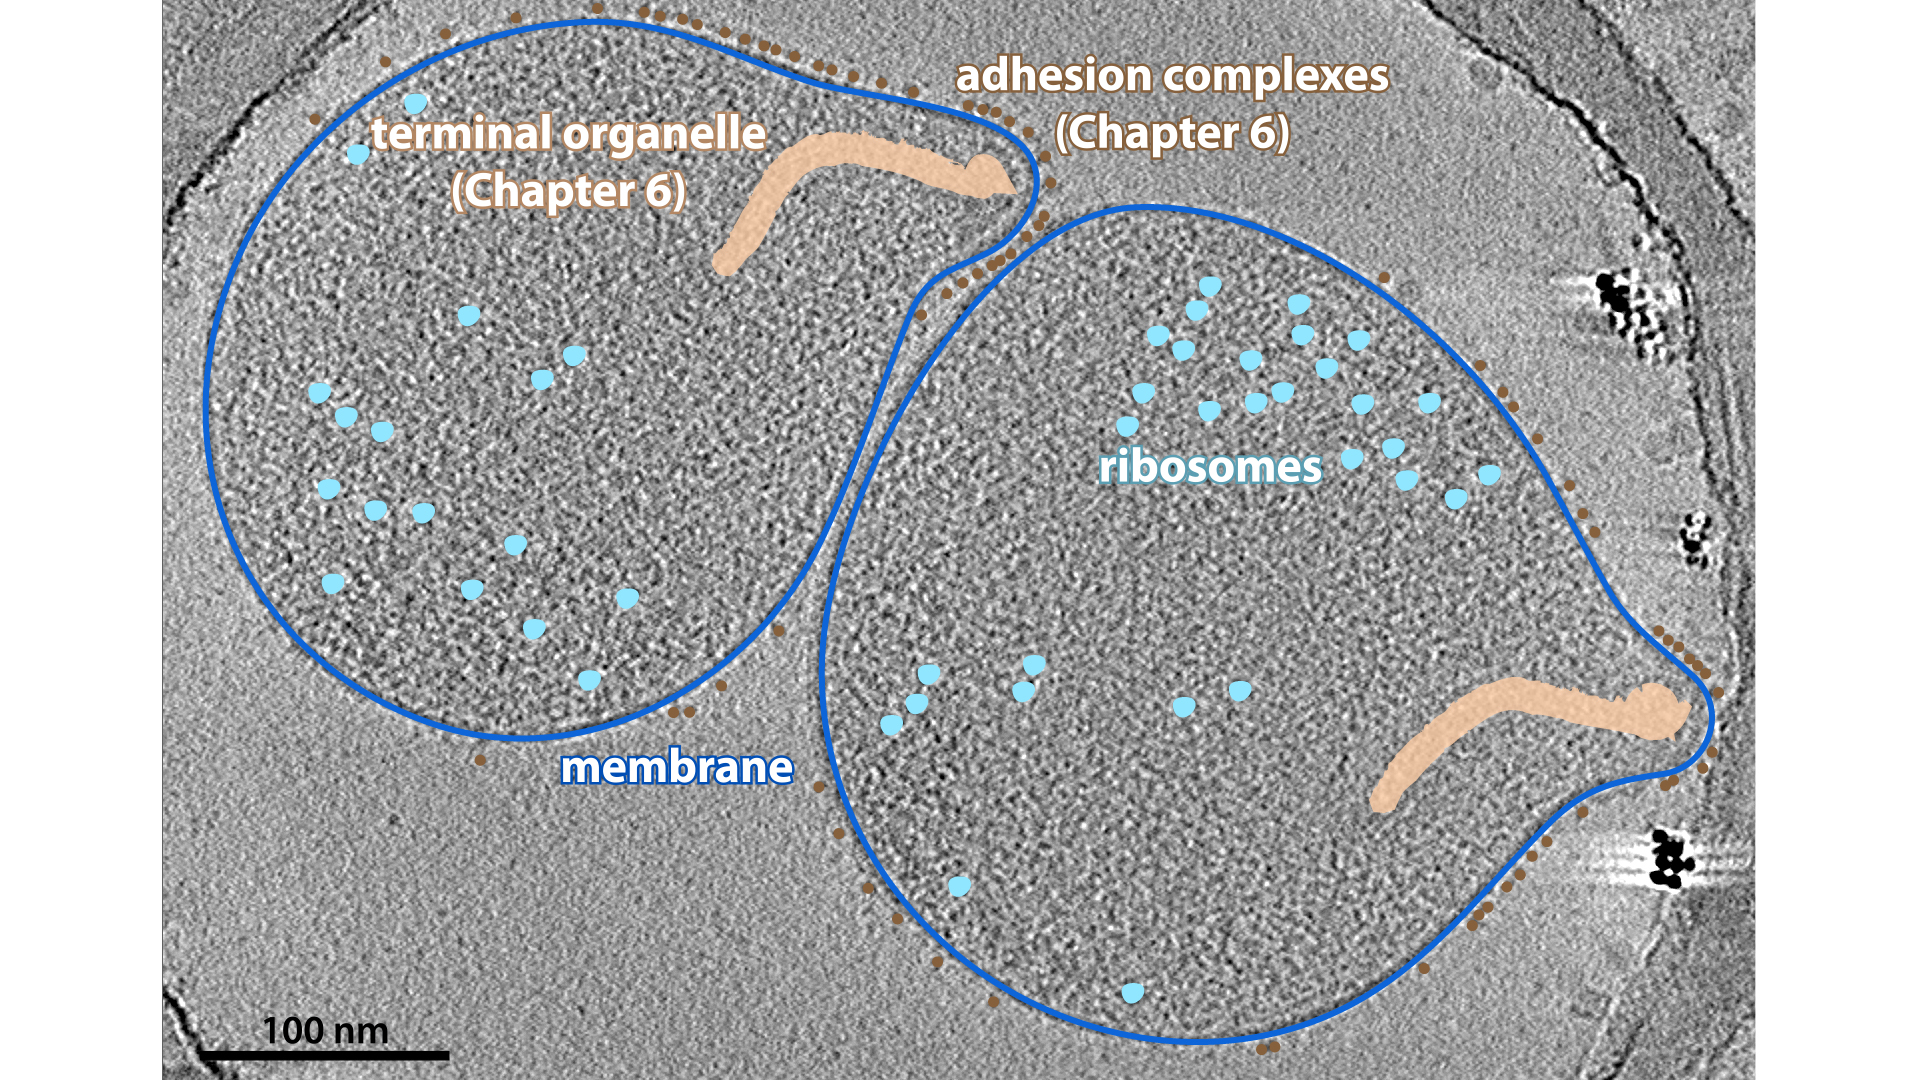
\includegraphics{img/02_static/2_1_Mgenitalium}

\hypertarget{N._maritimus}{\subsection{Nitrosopumilis
maritimus}\label{N._maritimus}}

In Nitrosopumilis maritimus, S-layer proteins form hexagonal rosettes
that in turn pack into a hexagonal lattice.

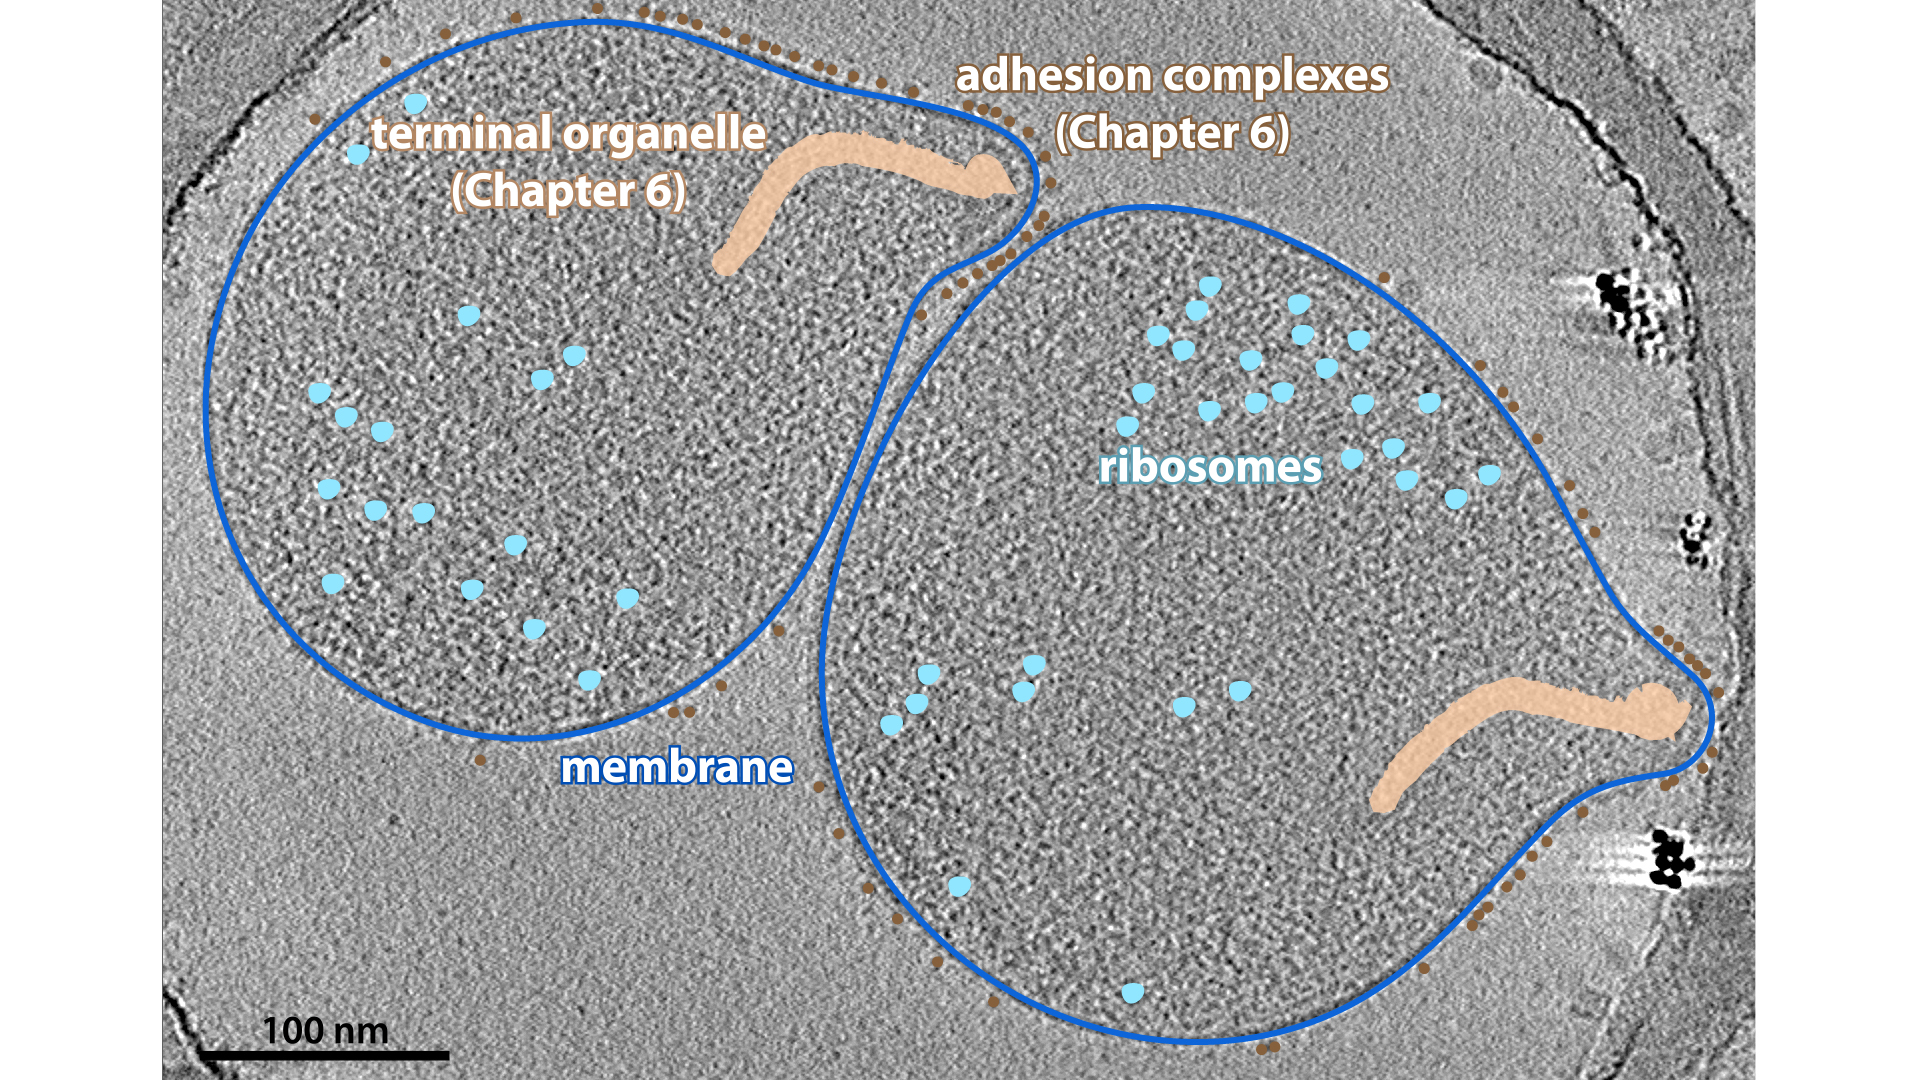
\includegraphics{img/02_static/2_1_Mgenitalium}

\hypertarget{Methanoregula_formicica}{\subsection{Methanoregula
formicica}\label{Methanoregula_formicica}}

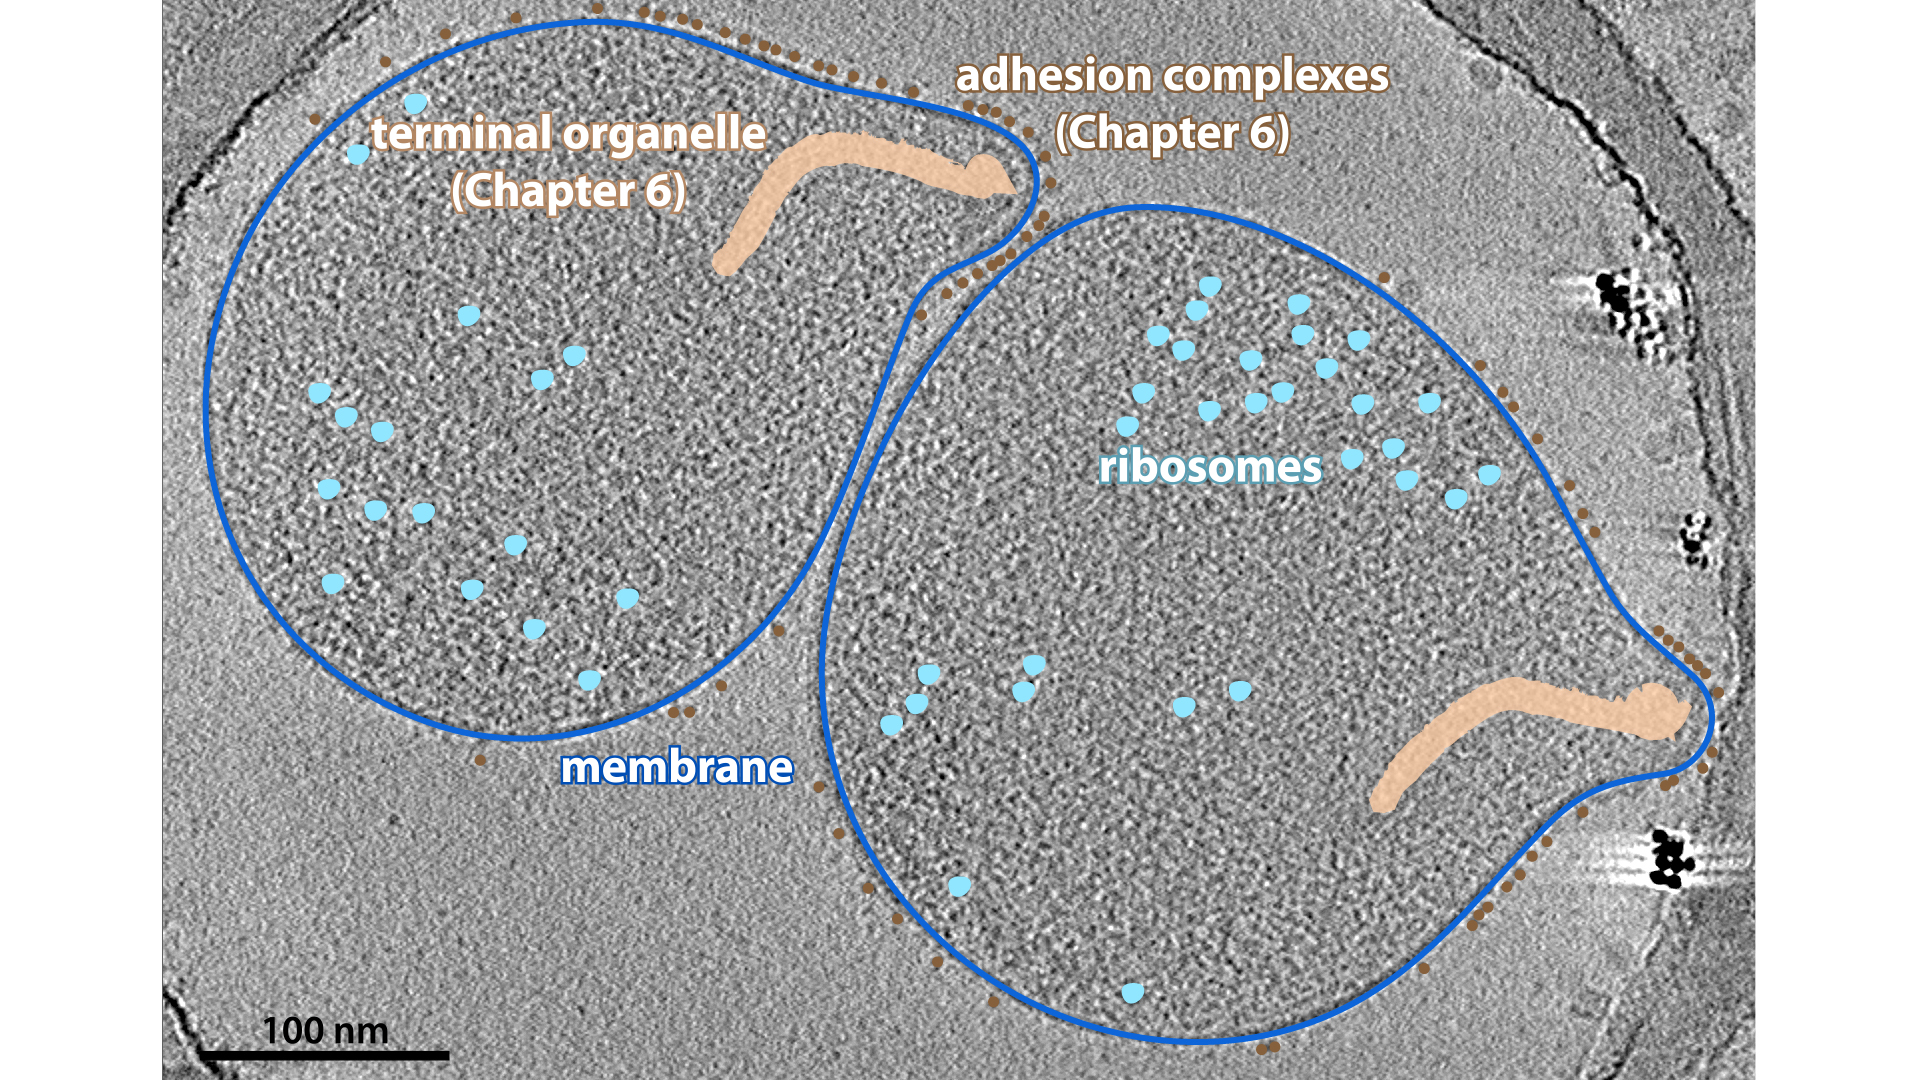
\includegraphics{img/02_static/2_1_Mgenitalium}

\section{Methanospirillum hungatei}\label{methanospirillum-hungatei}

Why stop with a single layer of protein? For proof that Nature is
endlessly inventive, consider this Methanospirillum hungatei cell. These
archaea encase themselves in an S-layer, and then an additional protein
layer that forms a highly impermeable sheath. The sheath is also very
resistant to pressure, which could be important in the cells' line of
work. M. hungatei were discovered in sewage, where they break down
organic waste, producing methane. One theory is that the sheath acts as
a pressure regulator; when enough methane builds up inside the cell, the
pressure expands the sheath, opening its pores wide enough to allow the
methane to dissipate and new metabolic substrates like hydrogen and
carbon dioxide to enter.

The rules of architecture remain the same, though. Just as in the
bacterial cell wall, sheath polymers are arranged as hoops perpendicular
to the long axis of the rod-shaped cell. The ends of the sheath, as you
can see, are special, with multiple protein layers stacking into a thick
plug. Cells divide within the sheath, and long chains of cells in a
continuous sheath are often observed.

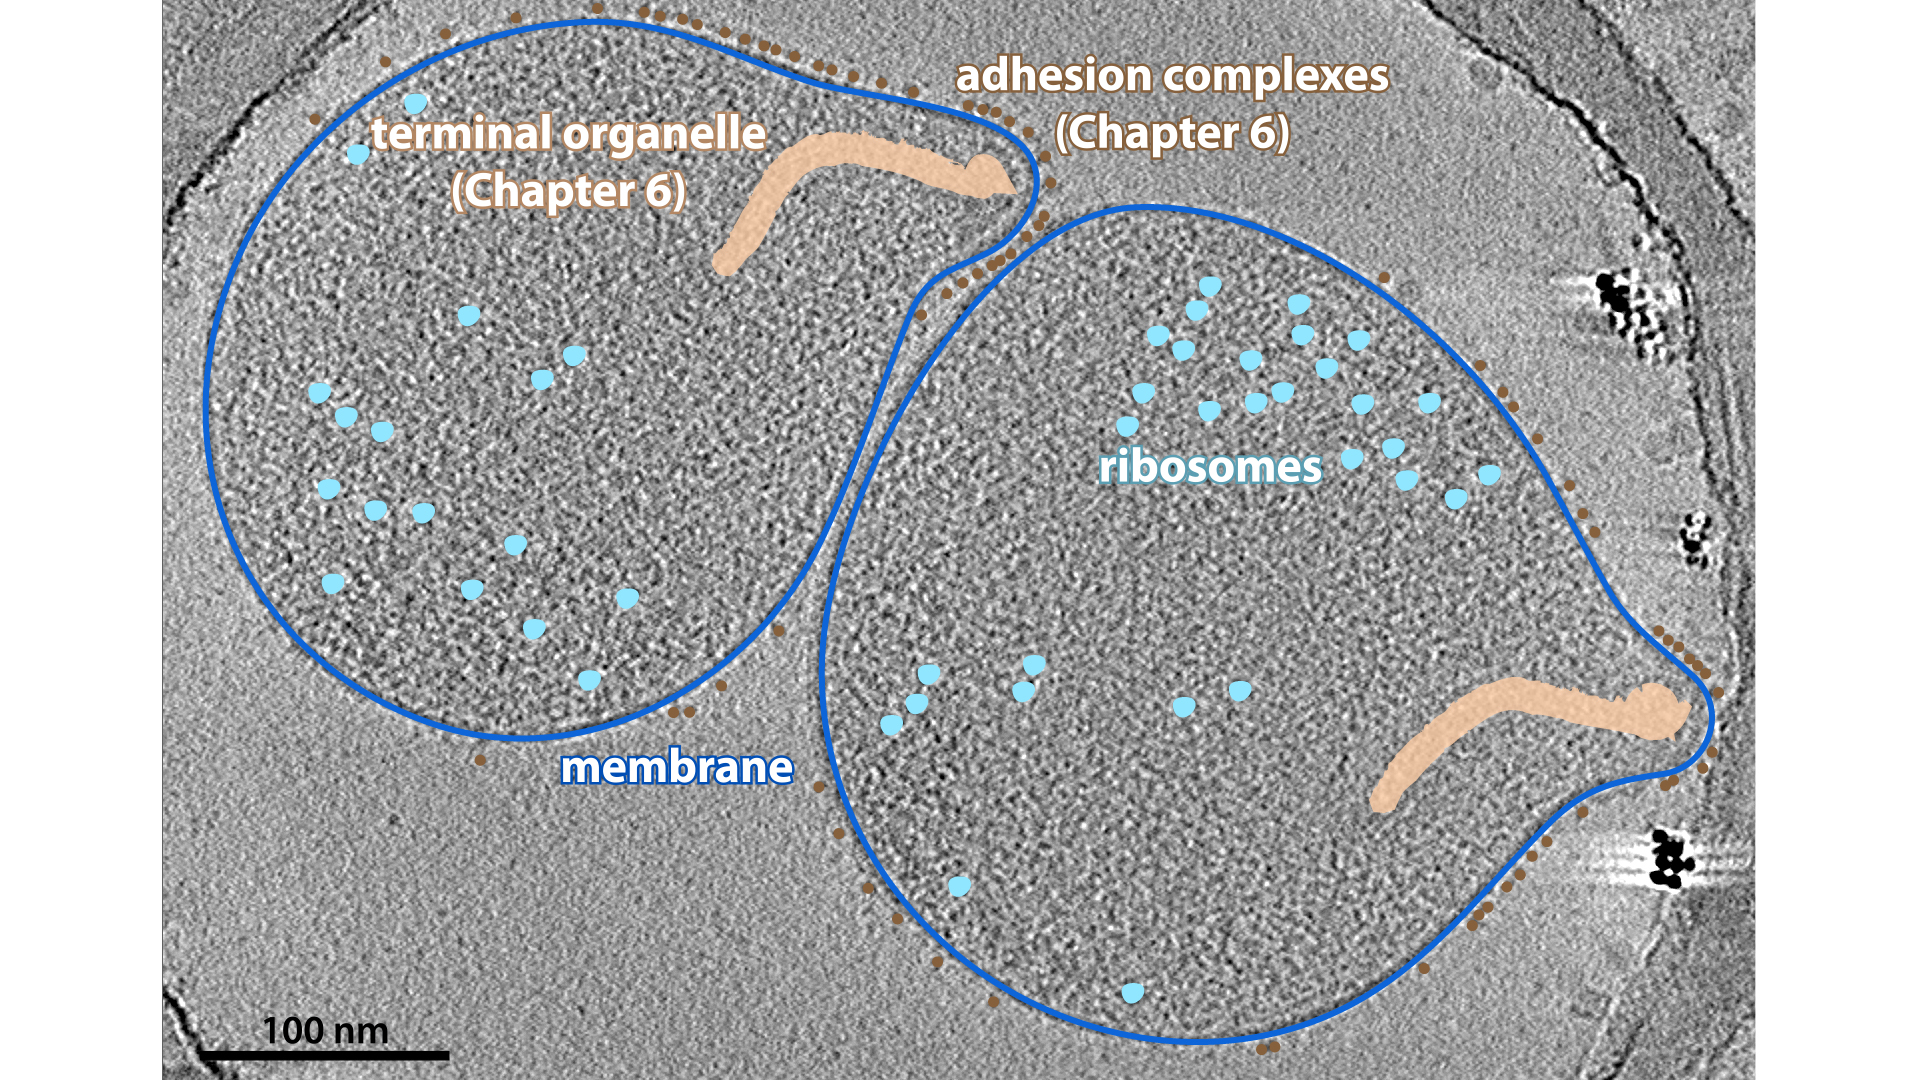
\includegraphics{img/02_static/2_1_Mgenitalium}

\section{Haloarcula argentinensis}\label{haloarcula-argentinensis}

All the layers we've just discussed collectively make up the container,
or envelope, of a cell. As you've seen, different species use different
combinations of these components to form their envelopes; the only
constant is the cytoplasmic (or inner, for diderms) membrane. Before we
move on, let's talk briefly about what these envelopes contain. In
addition to water and small molecules, you've already seen some large
protein complexes like motility machineries. You've also seen the
ribosomes -- the protein/RNA complexes responsible for translation. But
you might have been surprised not to see something else: DNA. The
replicating molecule containing the instructions for the life of the
cell is of paramount importance but often invisible by microscopy. But
not always.

Thin filaments of DNA, only about 2 nm wide, blend in with the dense
cytoplasm of the cell. When a cell lyses, though, its cytoplasm diffuses
into the environment and the DNA filaments stand out against the
now-much-reduced background. You can get an idea of the sheer abundance
of DNA in a cell from this Haloarcula argentinensis where the envelope
has ruptured and the contents are spilling out.

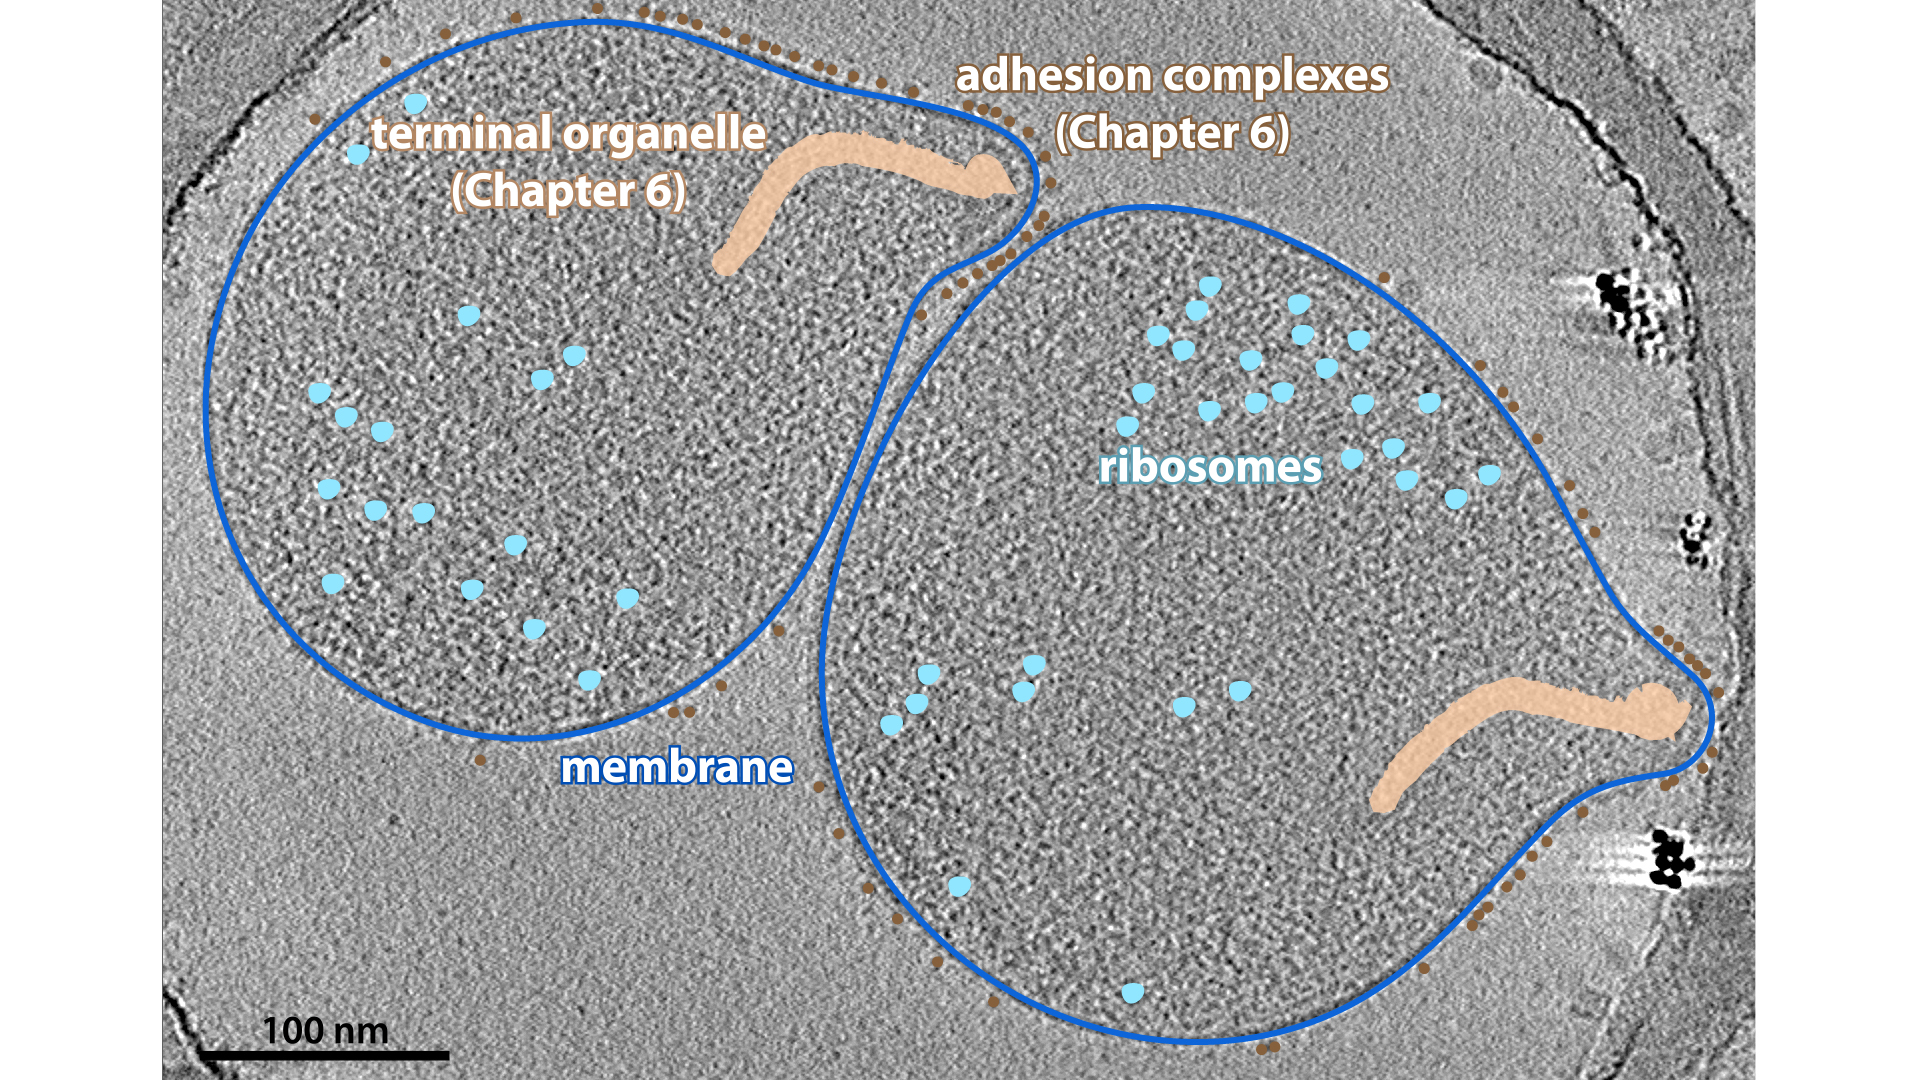
\includegraphics{img/02_static/2_1_Mgenitalium}

\section{Bdellovibrio bacteriovorus}\label{bdellovibrio-bacteriovorus}

Cells contain enormous amounts of DNA. The single, circular chromosome
of this Bdellovibrio bacteriovorus cell contains 3,782,950 individual
base pairs, which means that if the circle were cut and laid out as a
long piece, it would be about one thousand times longer than the cell
itself. To fit and function inside the cell, the chromosome has to be
extraordinarily organized and packed, a feat we still don't understand.
You can see some of this packing in nearly every cell: the center of the
cell tends to have very few large macromolecular complexes like
ribosomes, because they're excluded by the densely-packed chromosome(s).
Watch out for these ribosome-excluding zones in the rest of the book;
they indicate the location of the bulk of the cell's DNA. Since bacteria
and archaea don't enclose their DNA in a subcellular membrane, we don't
call this region a nucleus (the ``karyon'' that defines eukaryotes).
Instead, we use the term nucleoid to describe the cytoplasmic region
where most of the DNA is concentrated.

At times, the nucleoid becomes easier to see. Imagine that you want to
decrease gene expression in your cell. Don't worry yet about why --
we'll discuss that in Chapter 8 -- for now, just think about how. One
approach is simply to pack the chromosome so tightly that the
transcriptional machinery can't access the genes. That's what this cell
is doing, condensing its nucleoid into a dense twisted braid we can
easily visualize.

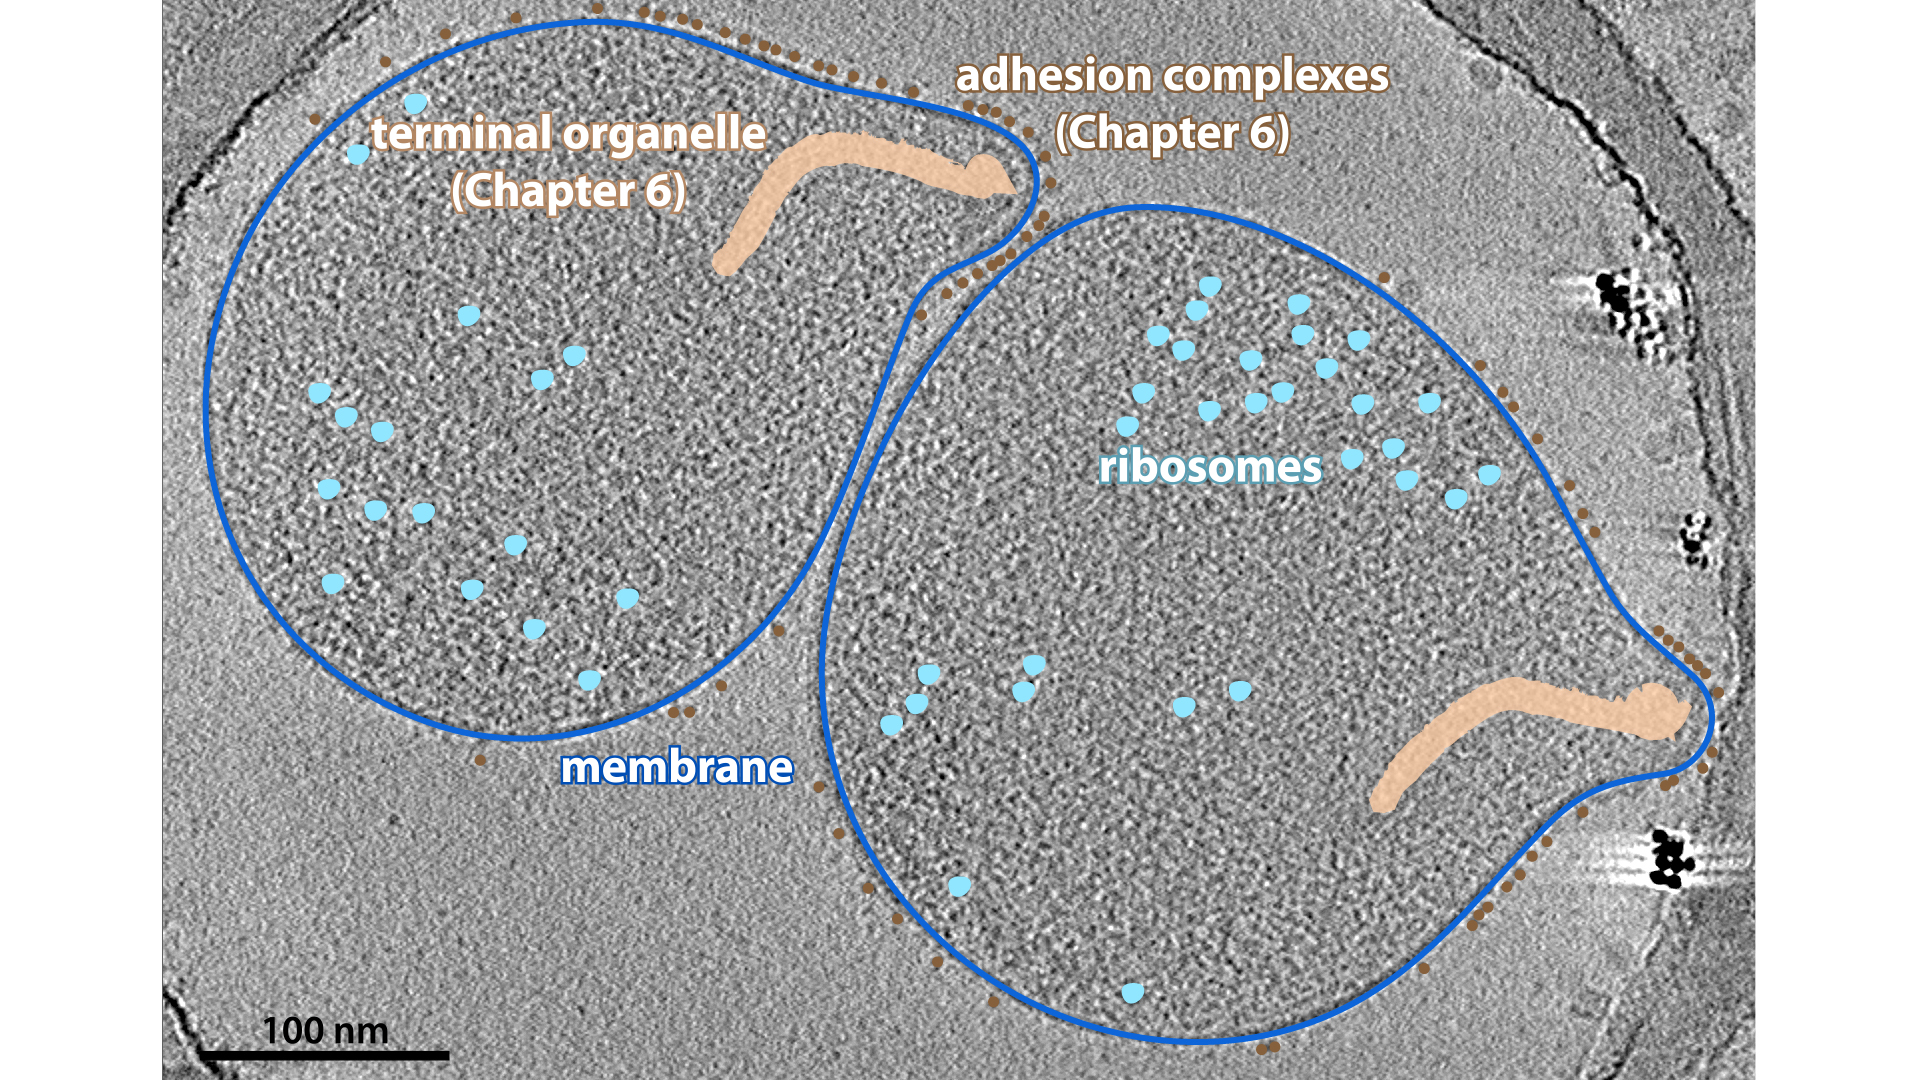
\includegraphics{img/02_static/2_1_Mgenitalium}

\bibliography{book.bib,packages.bib}



\end{document}
